\documentclass[12pt]{article}

\usepackage[utf8]{inputenc}
\usepackage[T1]{fontenc}
\usepackage[english]{babel}
\usepackage{geometry}
\geometry{margin=2.5cm}
\usepackage{amsmath}
\usepackage{capt-of}
\usepackage{booktabs}
\usepackage{longtable}
\usepackage{ltcaption}
\usepackage{multirow}
\usepackage{array}
\usepackage{tabularx}
\usepackage{colortbl}
\usepackage{graphicx}
\usepackage{xcolor}
\usepackage{eso-pic}
\usepackage{tikz}
\usepackage{authblk}
\usepackage{pdflscape}
\usepackage{afterpage}
\usepackage{float}

\usepackage[backend=biber,style=numeric,sorting=none]{biblatex}
\addbibresource{references.bib}
\appto\bibsetup{\sloppy}

\usepackage{xurl}
\usepackage[
  unicode=true,
  colorlinks=true,
  linkcolor=blue,
  citecolor=blue,
  urlcolor=blue,
  breaklinks=true
]{hyperref}
\usepackage{cleveref}

\crefname{table}{Table}{Tables}
\Crefname{table}{Table}{Tables}

\usetikzlibrary{positioning,backgrounds,fit,shapes,calc,matrix}
\usepackage{csquotes}
\usepackage{tocloft}

\renewcommand{\cfttoctitlefont}{\Large\bfseries}
\setlength{\cftbeforetoctitleskip}{0pt}
\setlength{\cftaftertoctitleskip}{1em}

\renewcommand\_{\texttt{\detokenize{_}\allowbreak}}

% ---------------------------------------------------------------------------
% Corpus-level figures — SINGLE SOURCE OF TRUTH for the manuscript AND the SI.
% Update these macros (and regenerate the input tables/figures) when a new
% database version is released; do not hard-code corpus numbers in the text.
% ---------------------------------------------------------------------------
\newcommand{\CCFarticles}{283{,}964}      % articles in the corpus
\newcommand{\CCFsentences}{9{,}908{,}776} % two-sentence analytical units
\newcommand{\CCFsentApprox}{9.9}          % ditto, millions (approx, one decimal)
\newcommand{\CCFembeddings}{10{,}192{,}740}% rows of CCF_sentence_embeddings
\newcommand{\CCFembedApprox}{10.19}        % ditto, millions (approx)
\newcommand{\CCFnewspapers}{22}           % distinct newspaper titles
\newcommand{\CCFyearfirst}{1978}
\newcommand{\CCFyearlast}{2026}
\newcommand{\CCFnyears}{48}               % elapsed span: yearlast - yearfirst
                                          % (Feb 1978 -> Jul 2026), not the count
                                          % of calendar years touched
\newcommand{\CCFenshare}{83.4}            % share of English units (%)
\newcommand{\CCFfrshare}{16.6}            % share of French units (%)
% Version-specific deposit identifiers and sizes (update on each release)
% One version number for all three deposits (data SQL, data Parquet, code):
% they are released together and must never drift apart again.
\newcommand{\CCFversion}{2.1.0}
\newcommand{\CCFsqldoi}{10.5281/zenodo.22019287}     % PostgreSQL edition (version DOI)
\newcommand{\CCFparquetdoi}{10.5281/zenodo.22019288} % Parquet mirror (version DOI)
\newcommand{\CCFcodedoi}{10.5281/zenodo.22019289}     % code & documentation deposit
\newcommand{\CCFsqldoiConcept}{10.5281/zenodo.20346363}
\newcommand{\CCFparquetdoiConcept}{10.5281/zenodo.20346372}
\newcommand{\CCFcodedoiConcept}{10.5281/zenodo.21921214}
\newcommand{\CCFsqlsize}{40}              % GB, CCF_Database.tar
\newcommand{\CCFparquetsize}{17.5}        % GB, Parquet mirror


% Supplementary Information is compiled separately as
%   paper/CCF_Methodology/Latex/CCF_Methodology_SI.tex
% Table labels with the prefix ``S'' (S1--S11) refer to that document.
\title{\textbf{CCF Database: A Machine-Learning-Annotated Corpus of \CCFarticles{} Canadian Climate Articles (\CCFyearfirst{}--\CCFyearlast{})}}

\author[1]{Antoine Lemor\thanks{antoine.lemor@umontreal.ca}}
\author[2]{Alizée Pillod\thanks{alizee.pillod@umontreal.ca}}
\author[2]{Matthew Taylor\thanks{matthew.taylor@umontreal.ca}}
\author[2]{Richard Nadeau\thanks{richard.nadeau@umontreal.ca}}
\affil[1]{Université de Sherbrooke}
\affil[2]{Université de Montréal}

\date{}

\setcounter{secnumdepth}{-1}  % no section numbering (Scientific Data requirement)
\tolerance=800
\emergencystretch=3em
\begin{document}

\maketitle
\thispagestyle{empty}


\begin{abstract}
\noindent
News media shape how societies perceive and respond to climate change, yet fine-grained analysis remains hindered by fragmented corpora and ad hoc coding schemes. The Canadian Climate Framing (CCF) database answers both with a large-scale bilingual annotated corpus and a generalizable annotation framework. It covers \CCFarticles{} climate-related articles from \CCFnewspapers{} Canadian news outlets (\CCFyearfirst{}--\CCFyearlast{}), processed into \CCFsentences{} two-sentence units (\CCFenshare{}\% English, \CCFfrshare{}\% French). Each unit carries 65 hierarchical binary annotations spanning eight main frames, actors, events, solutions, tone, geography, and urgency, produced by 128 BERT and CamemBERT classifiers trained on 4{,}000+ expert-coded sentences. Against a 1{,}000-sentence gold standard double-coded by an independent annotator (Cohen's $\kappa$ $=$ 0.596, Krippendorff's $\alpha$ $=$ 0.698, Gwet's AC1 $=$ 0.894), the classifiers reach a pooled macro $F_1$ of 0.866 (mean per-category macro $F_1$ $=$ 0.773), and every category carries an A/B/C reliability tier. The database---sentence-level annotations, per-article aggregations, and \CCFembeddings{} BAAI/bge-m3 embeddings in six relational tables---is openly released on Zenodo (CC-BY~4.0) as a PostgreSQL edition and an Apache Parquet mirror, refreshed roughly every six months by the CCF Observatory.
\end{abstract}

\newpage

\section{Background \& Summary}

On February 18, 1978, \textit{The Globe and Mail} ran a story headlined ``Some think it's warming up'' that reported on a survey of leading climate experts. Interestingly, almost half a century ago, the article already laid out for its readers what have since become the well-established root causes of climate change:
\begin{quote}
``The concern is that possible warming, the so-called `greenhouse effect,' is generally associated with the increase of carbon dioxide in the atmosphere by the burning of fossil fuels.''
\end{quote}
This excerpt clearly embodies the role the media play in informing society and citizens, who often lack direct access to academic research. At the same time, the media also reflect the social and political realities of the country they cover. Indeed, while some newspapers choose to relay the voices of scientists, others choose to report the controversies, so that the media both inform and reflect political and social realities. Research shows that media shape not only what people think about but also how they think about it, with effects on both public opinion and political agendas \autocite{scheufele_framing_2007, walgrave_contingency_2006}. The media are accordingly not a neutral arena for public debate around climate change. Instead, they actively participate in defining and constructing the problems under discussion \autocite{cohen_folk_1972, trevino_media_2018}. Moreover, while digital and social media have grown in prominence, newspapers remain a foundational source of information that continues to shape public discourse and to influence other media formats \parencite{bastos_shares_2015, casero-ripolles_impact_2020}. Studying print media therefore provides a vantage point on a traditional and still highly influential channel of climate communication. Most importantly, it allows for long-term historical comparison, including periods that predate the rise of social media.

The excerpt above was drawn from the oldest article of the \emph{Canadian Climate Framing (CCF)} database, which we introduce in this Data Descriptor. The CCF database is a machine-learning-preprocessed corpus of \CCFarticles{} climate-related newspaper articles published between \CCFyearfirst{} and \CCFyearlast{} across \CCFnewspapers{} major Canadian news outlets, accompanied by a rigorous, theoretically grounded annotation framework that we release alongside the data. The corpus contains \CCFsentences{} two-sentence analytical units, all annotated within a 65-category hierarchical coding scheme. Because Canadian newspaper articles are protected by copyright, the deposit does not redistribute the raw sentence text of the corpus at large (the sole, clearly bounded exception---the expert-coded training and gold-standard sentences---is documented in Data Records). What is shared instead is (i) the 65-category hierarchical annotation framework---a theoretically grounded coding scheme that integrates main frames, actors, events, solutions, emotional tone, geographic focus, and urgency into a single sentence-level taxonomy---and (ii) the full output of an intensive annotation pipeline built around that framework: 65 binary sentence-level labels per analytical unit, the named-entity extractions (persons, organizations, locations), the article-level aggregates and full metadata (newspaper, date, title, author, page number), the per-category reliability tiers, and the BAAI/bge-m3 sentence embeddings (\CCFembedApprox{}~million 1024-dimensional vectors). The breadth of the annotation scheme and the embedding layer together make the deposit fully analysable at the sentence level without requiring access to the raw text. By focusing on the Canadian press, this database constitutes a historically influential source of climate information.

Canada offers a particularly compelling case for studying climate discourse. Its federal structure, bilingual culture, and vast territory create a microcosm of the diversity---and contradictions---found globally. While Canada is highly vulnerable to the impacts of climate change \autocite{lulham_canada_2023}, it remains significantly dependent on fossil-fuel extraction and other resource-based industries \autocite{natural_resources_canada_energy_2025}. This creates structural tensions between environmental protection and economic interests. Some provinces, notably Quebec and British Columbia, tend to adopt more progressive climate policies, whereas others with resource-intensive economies are more cautious or resistant \autocite{harrison_struggle_2010}. This combination of political decentralization, linguistic duality, and regional economic variation produces diverse policy approaches and, in turn, shapes how climate change is discussed in the media. Yet systematic analysis of climate communication in Canada and elsewhere has long been constrained by methodological obstacles: until recently, large-scale corpus collection and precise, reproducible content analysis were virtually impossible. Supplementary Table~S1 provides an overview of prior studies in this area, highlighting their scope, focus, and coverage. The dominant pattern is one of corpora restricted to a few outlets, short observation windows, and English-language sources.

The CCF Database was designed to address four major limitations in previous research on climate change media coverage in Canada. First, the CCF draws on a larger set of news outlets and articles, comprising \CCFarticles{} articles from \CCFnewspapers{} news outlets with substantial representation for each outlet. Previous studies generally relied on smaller corpora and a limited number of newspapers, thereby capturing a narrower media landscape. Second, the CCF spans nearly five decades, providing a broader temporal perspective than most existing studies, which often focus on short periods or extend only from the late 1980s to the 2010s. Third, while climate attitudes vary significantly across regions \autocite{hatch_what_2025}, regional climate coverage remains understudied. Existing studies generally focus on nationally circulating newspapers---most commonly \textit{The Globe and Mail}, \textit{National Post}, and \textit{Toronto Star}---and rarely compare a large set of provinces and territories. The CCF therefore includes a wide range of regional newspapers. Finally, the CCF reflects Canada’s linguistic diversity through a bilingual corpus that includes a substantial share of French-language content (\CCFenshare{}\% English, \CCFfrshare{}\% French), with francophone outlets both inside and outside Quebec. While Canada is officially bilingual, previous research has largely excluded French-language media from analysis. Two studies, in particular, have examined francophone coverage: \textcite{young_comparing_2012}, comparing climate coverage between French-language outlets from Quebec and English-language outlets from the rest of Canada, and \textcite{king_how_2019}, analysing climate change's public-health framing with partial inclusion of Quebec.

Methodologically, the CCF database is the first climate media corpus to offer sentence-level annotations derived from supervised machine learning and natural language processing (NLP). Unlike unsupervised approaches such as topic modelling, which remain dominant in the field, the CCF methodology relies on transformer-based classifiers (BERT for English, CamemBERT for French) trained on over 4,000 manually expert-coded sentences. NLP enables scholars to examine much larger corpora in far less time, opening new avenues for systematic inquiry \autocite{swarnakar_nlp_2021, schafer_computational_2023, hirsbrunner_computational_2024}. However, as summarised in Supplementary Table~S1, when climate researchers do employ NLP it is most often to identify key actors through named-entity recognition, to detect stance, or to conduct sentiment analysis, which tend only to map actors, tone, or evaluative direction rather than interpretive structures. The dominant computational approach in the field is still unsupervised topic modelling, where topics are treated as proxies for frames---an assumption that \textcite{nicholls_computational_2024} and \textcite{otmakhova_media_2024} flag as problematic, as topics are too narrow to capture the defining features of frames, which, following \textcite{entman_framing_1993}, require identifying a problem, specifying causal interpretations, moral evaluations, and possible solutions. By contrast, the supervised approach adopted in the CCF Database enables the identification of frames, actor types, events, solution strategies, and emotional tone with a level of semantic precision that unsupervised methods cannot achieve. Only a few studies have applied comparable transformer-based models in this domain: \textcite{luo_detecting_2021} trained a single BERT classifier to analyse the evolution of climate partisanship in U.S.\ media; \textcite{meddeb_counteracting_2022} used a CamemBERT model to detect climate misinformation in French news; \textcite{frermann_conflicts_2023} fine-tuned transformer models to detect narrative roles (conflict, villain, resolution) in media articles on three issues including climate change; \textcite{badullovich_manual_2026} benchmarked a RoBERTa classifier against zero-shot LLMs on issue and rhetorical frames in climate change editorials published in \textit{Nature} and \textit{Science}. None of these works, however, have trained and deployed a comparable suite of transformer models to systematically annotate climate-related media coverage at the scale, breadth, and bilingual coverage of the CCF database.

Validated against an independent gold standard of 1,000 expert-coded sentences whose reliability was confirmed through double-coding (Cohen's $\kappa$ = 0.596, Krippendorff's $\alpha$ = 0.698, Gwet's AC1 = 0.894, on the blind-coding phase of sentences 601--1000), the CCF trained models attain a pooled macro F1 score of 0.866 across the 65 annotation categories (0.773 when the 65 per-category macro F1 scores are averaged without pooling; both quantities are defined and discussed in the Technical Validation section). In addition, named-entity recognition (NER) was applied to extract persons, organisations, and locations mentioned in the articles, and the entire corpus was embedded with the BAAI/bge-m3 multilingual encoder so that semantic-similarity queries can be issued directly against the deposited database. With 128 BERT and CamemBERT classifiers covering frames, actors, events, solutions, and emotional tone, the CCF database fills a clear methodological gap by introducing a supervised NLP approach capable of detecting multiple analytical dimensions at scale, and the absence of raw text in the deposit is offset by the depth of the annotation: every sentence carries 65 binary labels, a deduplicated NER signature, and a 1024-dimensional embedding, so researchers can run frame-based, actor-based, and semantic queries directly on the deposited tables. This technical paper presents the methodology underlying the CCF database and its structure. The remainder of the document outlines the full workflow (data acquisition and preprocessing, model training, validation, and database enrichment) and offers the conceptual rationale and practical steps necessary for researchers wishing to work with the CCF database or to adapt its methodology elsewhere.

\afterpage{%
\begin{landscape}
\pagestyle{empty}
\vspace*{\fill}

\begin{figure}[h!]
\centering
\resizebox{0.95\linewidth}{!}{%
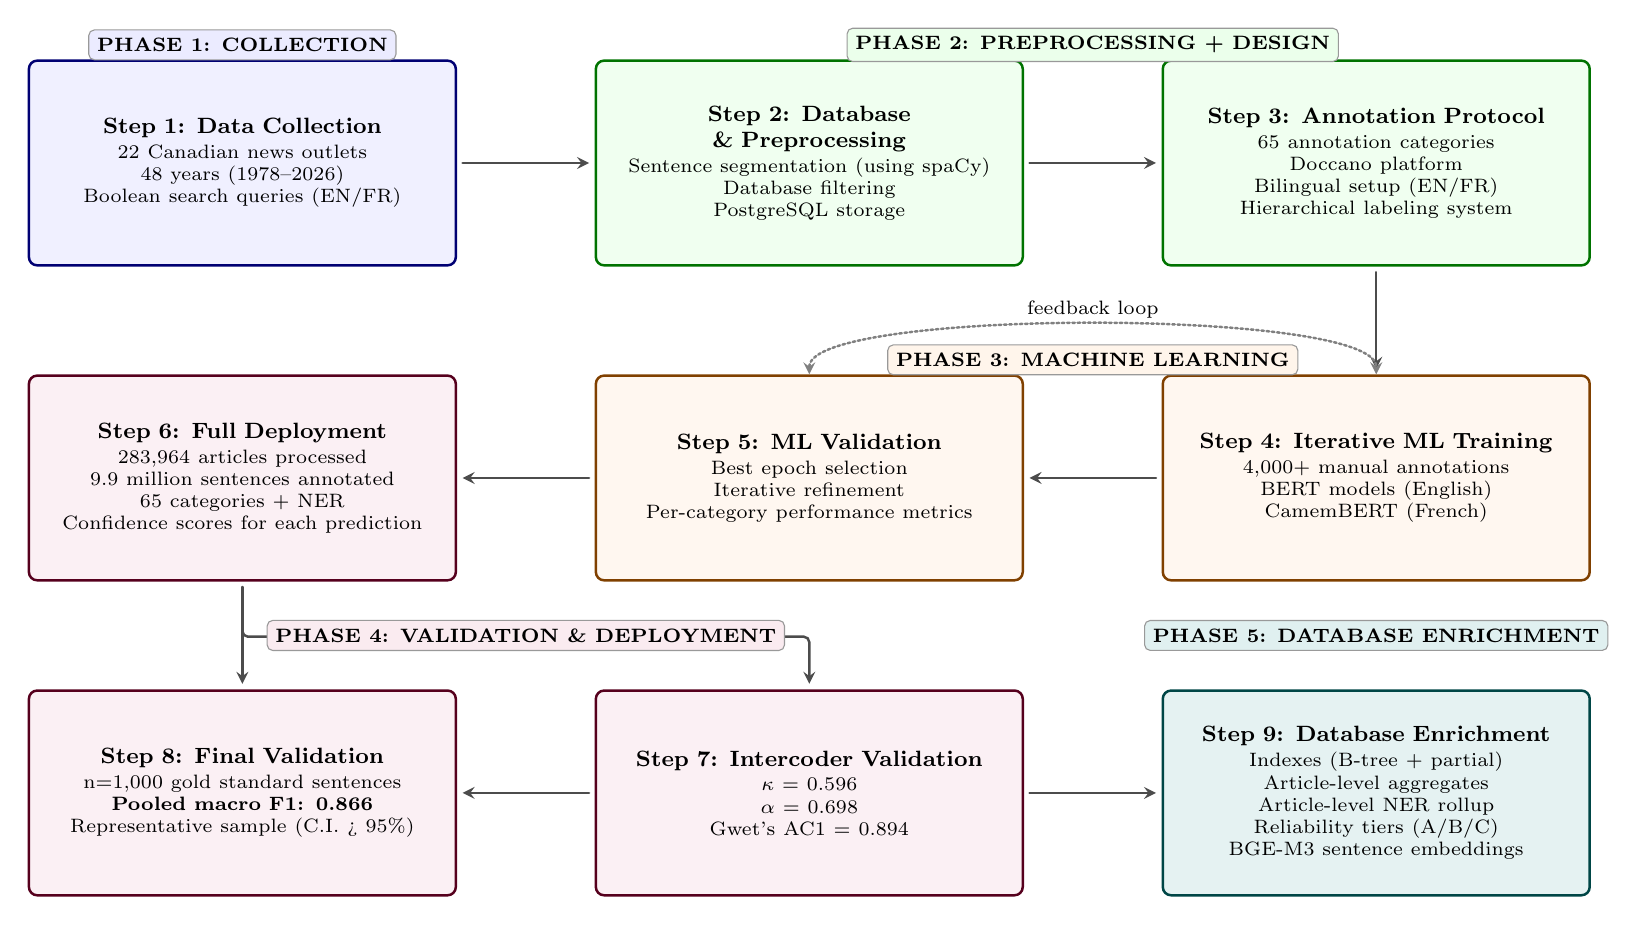
\begin{tikzpicture}[
    box/.style = {
        rectangle,
        draw=black!50,
        line width=0.9pt,
        rounded corners=3pt,
        minimum width=5.2cm,
        minimum height=2.6cm,
        align=center,
        font=\footnotesize,
        text width=5cm,
        inner sep=6pt,
        fill opacity=1
    },
    collect/.style = {box, fill=blue!6,   draw=blue!45!black},
    process/.style = {box, fill=green!6,  draw=green!45!black},
    train/.style   = {box, fill=orange!6, draw=orange!50!black},
    valid/.style   = {box, fill=purple!6, draw=purple!45!black},
    pending/.style = {box, fill=gray!6,   draw=gray!60, line width=0.9pt, dashed, text=gray!60},
    deploy/.style  = {box, fill=purple!6,    draw=purple!45!black},
    enrich/.style  = {box, fill=teal!10,  draw=teal!55!black},
    arrow/.style      = {->, line width=0.9pt, >=stealth, draw=black!70, rounded corners=2pt, shorten >=2pt, shorten <=2pt},
    dasharrow/.style  = {->, line width=0.9pt, >=stealth, draw=black!55, densely dashed, rounded corners=2pt, shorten >=2pt, shorten <=2pt},
    feedbackarrow/.style = {<->, line width=0.9pt, >=stealth, draw=black!50, densely dotted},
    phaselabel/.style = {rectangle, draw=black!40, rounded corners=2pt, inner sep=3pt, font=\scriptsize\bfseries},
    line cap=round, line join=round
]

\def\hspace{7.2}
\def\vspace{4}

\node[collect] (datacoll) at (0,0) {
    \textbf{Step 1: Data Collection}\\[1pt]
    \scriptsize
    \CCFnewspapers{} Canadian news outlets\\
    \CCFnyears{} years (\CCFyearfirst{}--\CCFyearlast{})\\
    Boolean search queries (EN/FR)\\[1pt]
};

\node[process] (database) at (\hspace,0) {
  \textbf{Step 2: Database \& Preprocessing}\\[1pt]
  \scriptsize
  Sentence segmentation (using spaCy)\\
  Database filtering\\
  PostgreSQL storage\\[1pt]
};

\node[process] (protocol) at (2*\hspace,0) {
    \textbf{Step 3: Annotation Protocol}\\[1pt]
    \scriptsize
    65 annotation categories\\
    Doccano platform\\
    Bilingual setup (EN/FR)\\
    Hierarchical labeling system\\[1pt]
};

\node[train] (iterml) at (2*\hspace,-\vspace) {
    \textbf{Step 4: Iterative ML Training}\\[1pt]
    \scriptsize
    4,000+ manual annotations\\
    BERT models (English)\\
    CamemBERT (French)\\[1pt]
};

\node[train] (verification) at (\hspace,-\vspace) {
    \textbf{Step 5: ML Validation}\\[1pt]
    \scriptsize
    Best epoch selection\\
    Iterative refinement\\
    Per-category performance metrics\\[1pt]
};

\node[deploy] (fullannotation) at (0,-\vspace) {
    \textbf{Step 6: Full Deployment}\\[1pt]
    \scriptsize
    \CCFarticles{} articles processed\\
    \CCFsentApprox{}~million sentences annotated\\
    65 categories + NER\\
    Confidence scores for each prediction\\[1pt]
};

\node[valid] (validation) at (0,-2*\vspace) {
    \textbf{Step 8: Final Validation}\\[1pt]
    \scriptsize
    n=1,000 gold standard sentences\\
    \textbf{Pooled macro F1: 0.866}\\
    Representative sample (C.I. > 95\%)\\[1pt]
};

\node[valid] (intercoder) at (\hspace,-2*\vspace) {
    \textbf{Step 7: Intercoder Validation}\\[1pt]
    \scriptsize
    $\kappa$ = 0.596\\
    $\alpha$ = 0.698\\
    Gwet's AC1 = 0.894\\[1pt]
};

\node[enrich] (enrichment) at (2*\hspace,-2*\vspace) {
    \textbf{Step 9: Database Enrichment}\\[1pt]
    \scriptsize
    Indexes (B-tree + partial)\\
    Article-level aggregates\\
    Article-level NER rollup\\
    Reliability tiers (A/B/C)\\
    BGE-M3 sentence embeddings\\[1pt]
};

\draw[arrow] (datacoll.east) -- (database.west);
\draw[arrow] (database.east) -- (protocol.west);
\draw[arrow] (protocol.south) -- (iterml.north);
\draw[arrow] (iterml.west) -- (verification.east);
\draw[arrow] (verification.west) -- (fullannotation.east);

\draw[feedbackarrow]
    (verification.north) to[out=90,in=90, looseness=0.3]
    node[above, yshift=1pt, font=\scriptsize, fill=white, inner sep=1pt] {feedback loop}
    (iterml.north);

\draw[arrow] (fullannotation.south) -- (validation.north);
\draw[arrow] (fullannotation.south) -- ++(0,-0.7) -| (intercoder.north);
\draw[arrow] (intercoder.west) -- (validation.east);
\draw[arrow] (intercoder.east) -- (enrichment.west);

\node[phaselabel, fill=blue!8]   at (0,1.5)               {PHASE 1: COLLECTION};
\node[phaselabel, fill=green!8]  at (1.5*\hspace,1.5)     {PHASE 2: PREPROCESSING + DESIGN};
\node[phaselabel, fill=orange!8] at (1.5*\hspace,-2.5)    {PHASE 3: MACHINE LEARNING};
\node[phaselabel, fill=purple!8] at (0.5*\hspace,-1.5*\vspace)    {PHASE 4: VALIDATION \& DEPLOYMENT};
\node[phaselabel, fill=teal!12]  at (2*\hspace,-1.5*\vspace)    {PHASE 5: DATABASE ENRICHMENT};

\end{tikzpicture}
}
\caption{Methodological pipeline of the Canadian Climate Framing (CCF) project.}
\label{fig:methodology_overview}
\end{figure}
\vspace*{\fill}

\end{landscape}
}% end \afterpage

\section{Methods}

The CCF Database was built through a mixed-methods design that coupled large-scale data collection with state-of-the-art machine learning (ML). The resulting pipeline provides a systematic and reproducible framework for large-scale analysis of climate discourse that allows researchers to track how climate change is discussed, how narratives evolve over time, and who participates in the conversation.

Figure~\ref{fig:methodology_overview} presents the complete methodological pipeline and illustrates how the CCF Database was assembled from raw newspaper articles into a fully annotated database suitable for robust and reproducible climate communication research, both quantitative and qualitative. The pipeline combined human expertise with computational methods through an iterative human-in-the-loop machine learning procedure. This approach ensured both the scalability needed to process \CCFarticles{} climate-related articles and the accuracy required for rigorous academic research.

The methodology comprises five distinct phases: (1) the \emph{Collection Phase} involved systematic gathering of climate-related articles from \CCFnewspapers{} major Canadian news outlets using search queries resulting in \CCFarticles{} articles spanning \CCFyearfirst{}--\CCFyearlast{}; (2) the \emph{Preprocessing and Design} phase transformed raw text into structured data, including sentence segmentation, language verification, and development of a comprehensive 65-category annotation framework; (3) the \emph{Machine Learning} phase created and validated transformer-based machine learning models (BERT for English, CamemBERT for French) through iterative training with over 4,000 expert manual annotations; (4) the \emph{Validation and Deployment} phase ensured rigorous quality assurance by combining standard performance metrics with a human evaluation protocol based on an expert-coded gold standard that was independently double-coded by a second annotator to assess intercoder reliability, before deploying the trained models to annotate the complete corpus of \CCFsentApprox{}~million sentences; and (5) the \emph{Database Enrichment} phase consolidated the sentence-level output into a publication-ready relational system by adding four derived tables (article-level annotation aggregates, article-level named-entity rollups, per-category reliability tiers, and \CCFembedApprox{}~million BAAI/bge-m3 sentence-and-title embeddings indexed for approximate nearest-neighbour search), together with a complete index structure, so that the deposit can be queried directly without rewriting the same aggregation logic on every project.

\subsection{Phase 1 \& 2: Data collection, preprocessing, database creation and annotation protocol}

\subsubsection{Step 1: Data collection}

The CCF database was built through a systematic protocol to trace the evolution of climate discourse in Canada's bilingual print media, reaching back to the earliest available archives.

Articles were retrieved through university library access to three press databases: Factiva, Eureka.cc, and ProQuest Canadian Major Dailies. These platforms are the standard providers of full-text archives for Canadian newspapers and are routinely used in peer-reviewed media research \autocite{young_comparing_2012, king_how_2019, meddeb_counteracting_2022}. Each platform was queried independently with the same bilingual Boolean keywords (see Table~\ref{tab:boolean_queries} below) restricted to the selected outlets and to the full available time range (the 20 newspapers of the original collection; the CCF Observatory subsequently added the two public-broadcaster news sites through their own feeds), and duplicate articles appearing in more than one platform were collapsed at preprocessing time on the basis of newspaper, date, headline, and a 95\% fuzzy similarity of the article body (see \hyperref[subsec:step2_preprocessing]{Step~2}). Full bibliographic metadata are included in the deposit so that the corpus remains transparent and reproducible while staying within the bounds of copyrights. The design relies on the fair-dealing research exception in Canadian copyright law and the analogous fair-use research exception in U.S.\ law, both of which authorise non-consumptive, transformative use of copyrighted text for academic research; researchers with institutional access to Factiva, Eureka.cc, or ProQuest Canadian Major Dailies can recover the original text from the bibliographic coordinates.

A total of \CCFnewspapers{} news outlets---20 newspapers and, since the corpus came under the stewardship of the CCF Observatory, the two news websites of the Canadian public broadcaster (CBC.ca and Radio-Canada.ca, covered from 2023 onward)---are included in the corpus (see Supplementary Table~S2). The objective was to include both national and regional outlets in order to ensure broad geographic representation. Within this pool, newspapers were primarily chosen based on circulation levels \autocite{newspapers_canada_circulation_2015}, with the highest-circulating outlets retained. Additional criteria also informed the selection, including the desire to capture a range of political orientations and to build a bilingual corpus that reflects Canada's linguistic landscape. The corpus accordingly includes French-language outlets both inside and outside Quebec, together with one English-language outlet located in Quebec; this asymmetry mirrors the country's linguistic geography, in which Quebec is the only province with French as its sole official language while New Brunswick is officially bilingual and several other provinces---most notably northeastern Ontario along the Quebec border---host sizeable francophone communities. The final selection was also partly shaped by availability constraints. When the highest-circulating newspaper of a given province was unavailable, the next highest-circulating outlet was retained instead; for Prince Edward Island, Nunavut, and the Northwest Territories, no eligible newspaper was available for inclusion at all. Coverage windows are bounded by the access periods of the source aggregators: Le Droit is covered until December 2023, The Whitehorse Daily Star until May 2024, and Le Devoir and L'Acadie Nouvelle until March 2025, while all other outlets extend to the corpus cut-off of July 2026; Supplementary Table~S2 details the composition and per-outlet counts.

The corpus spans \CCFnyears{} years, from \CCFyearfirst{} to \CCFyearlast{}, with \CCFyearfirst{} marking the earliest article identified, quoted in the introduction of this paper. To identify climate-related articles, the authors used a transparent keyword-based filter with seven climate-domain terms per language (Table~\ref{tab:boolean_queries}). To be included in the data set, an article had to contain at least one of these keywords in its title or body. These queries yielded an initial corpus of over 300,000 articles. As with any keyword-based retrieval, the procedure imposes a recall ceiling: it cannot capture paraphrastic, metonymic, or strictly context-only mentions of climate change, and the deposit therefore covers articles that explicitly use one of the query terms rather than the broader set of articles that discuss climate change in some form. 

\begin{center}
\begingroup
\refstepcounter{table}\label{tab:boolean_queries}
\begin{minipage}{0.95\linewidth}
\centering
\setlength{\tabcolsep}{8pt}
\renewcommand{\arraystretch}{1.25}
\textbf{Table \thetable. Boolean queries used for article retrieval}
\vspace{0.5em}

{\fontsize{10}{12}\selectfont
\begin{tabular}{>{\raggedright\arraybackslash}p{2.8cm} >{\raggedright\arraybackslash}p{12cm}}
\toprule
\textbf{Language} & \textbf{Boolean Query} \\
\midrule
English & "global warming" OR "climate change" OR "climate disruption" OR "climate disturbance" OR "climate disturbances" OR "climate crisis" OR "greenhouse gas" \\
French & "réchauffement climatique" OR "réchauffement planétaire" OR "changement climatique" OR "changements climatiques" OR "dérèglement climatique" OR "crise climatique" OR "gaz à effet de serre" \\
\bottomrule
\end{tabular}
}
\end{minipage}
\endgroup
\end{center}

\subsubsection{Step 2: Preprocessing}
\label{subsec:step2_preprocessing}

The preprocessing phase transformed the raw data into a structured dataset suitable for machine learning. Each article was segmented into two-sentence contexts using language-specific spaCy models---\texttt{en\_core\_web\_lg} for English text and \texttt{fr\_dep\_news\_trf} for French text, both optimised for news content. Sliding windows with single-sentence overlaps were implemented to ensure complete coverage while maintaining semantic continuity throughout each article. This level of granularity supported machine-learning applications by increasing the size of the training dataset. More importantly, working at the (near-)sentence level was the only approach that allowed ex-post analysis to remain highly granular compared to paragraphs, where multiple frames, actors, or solutions can co-occur and become indistinguishable. Article-level variables could then be reconstructed with high granularity by aggregating sentence-level annotations (e.g., percentage of sentences in an article that mention a specific frame or actor), whereas paragraph-level annotations would have been less precise and more difficult to interpret.

Quality control measures were applied systematically throughout the data preparation pipeline. Duplicate articles were identified and removed with fuzzy string-similarity algorithms set to a 95\% threshold. Any article containing fewer than 100 words was also removed  to eliminate reader letters, which often did not provide enough material to identify the presence of a frame and did not qualify as a press article per se. However, all other types of text (opinion columns, letters to the editor, news articles, editorials, etc.) were retained. Regarding this matter, \textcite{lawrence_framing_2004} explains that it is precisely in editorials, or more generally in opinion texts, where journalistic standards are applied with a greater degree of flexibility, that the battle of framing is best observed. Articles published by external news agencies (for example, \textit{Agence France-Presse}, \textit{CanWest News Service}, \textit{Reuters}, or \textit{Bloomberg}) or by other newspapers not included in the analysis but which often belong to the same media conglomerate as the selected outlets (for example, \textit{the Financial Post}) were also retained. These republications were treated as aligned with the editorial direction of the host news outlet, and a republication did not contradict the objectives of the study since it indicated editorial interest in a topic concerning climate change. This process reduced the corpus to \CCFarticles{} unique articles. Duplicates of the same article appearing in different media outlets were deliberately kept, since their co-occurrence is itself an object of analysis when measuring media bubbles.

Language was then verified with the pre-trained fastText language-identification model \autocite{joulin_bag_2017, joulin_fasttext_2016}, in order to ensure consistent categorisation of bilingual content, and publication dates were standardised at the same step. This data preparation produced a clean, standardised corpus ready for machine learning and annotation, stored in two PostgreSQL tables: one with full metadata (titles, main text, authors, dates, and page numbers) and another with the processed sentence segments and their corresponding identifiers.

The resulting database is illustrated in Figure~\ref{fig:media_dist}, which displays the distribution of article counts by media (\CCFnewspapers{} outlets), while Figure~\ref{fig:year_counts} shows the total article counts per year across the full time span; the final months of 2026 are incomplete by construction, the corpus being cut off at 31~July~2026. The corpus is now maintained by the CCF Observatory, the continuous extraction--annotation pipeline described above, and is refreshed on Zenodo approximately every six months. Finally, Figure~\ref{fig:province_dist} presents the distribution of articles by province, based on the primary location of each outlet. This geographic breakdown shows the representativeness of the database across Canada, with \CCFenshare{}\% of sentence units in English and \CCFfrshare{}\% in French. The national outlets---\textit{The Globe and Mail}, the \textit{National Post}, the \textit{Toronto Star}, and the two public-broadcaster news sites---are omitted from the provincial breakdown because of their pan-Canadian scope; nevertheless, they account for 37.5\% of all articles.

\begin{figure}[p]
  \centering
  \begin{minipage}[t]{0.48\textwidth}
    \centering
    \includegraphics[width=\linewidth,height=0.32\textheight,keepaspectratio]{Figures/articles_by_media.png}
    \captionof{figure}{Distribution of articles by media.}
    \label{fig:media_dist}
  \end{minipage}\hfill
  \begin{minipage}[t]{0.48\textwidth}
    \centering
    \includegraphics[width=\linewidth,height=0.32\textheight,keepaspectratio]{Figures/articles_by_year.png}
    \captionof{figure}{Total number of articles per year.}
    \label{fig:year_counts}
  \end{minipage}

  \vspace{1em}

  \centering
  \includegraphics[width=\textwidth,height=0.5\textheight,keepaspectratio]{Figures/articles_by_province.png}
  \captionof{figure}{Distribution of articles by province.}
  \label{fig:province_dist}
\end{figure}

\subsubsection{Step 3: Annotation protocol}

The annotation framework constitutes the conceptual core of the CCF database. It comprises 65 categories organised into a hierarchical taxonomy designed to capture multiple dimensions of climate discourse at near-sentence granularity. The framework was developed through a combined theory-driven and data-driven procedure: it drew on established scholarship in framing, agenda-setting, climate communication, and social problems studies, and was refined inductively through iterative engagement with the corpus and extensive pretesting. The full taxonomy and operational definitions are reported in Supplementary Table~S3, while Table~\ref{tab:framework_summary} provides a compact overview of the framework's structure. The framework was organised around \emph{Primary Categories} corresponding to broad analytical dimensions, and \emph{Sub-categories} capturing internal distinctions within each \emph{Primary Category} (Table~\ref{tab:framework_summary}).

{\bfseries{Primary categories.}} The framework was organised around four primary analytic categories that structure the annotation protocol: \emph{Main Frames}, \emph{Actors/Messengers}, \emph{Events}, and \emph{Solutions} (Table~\ref{tab:framework_summary}). Drawing on climate communication research, these categories acknowledge that media coverage does more than describe the issue, since it also selects the interpretive lens through which it is read and understood, the actors who are granted voice, the events that anchor attention, and the courses of action that are put forward as plausible.

First, for \emph{Main Frames}, the authors built on the general framing tradition often associated with \textcite{entman_framing_1993}, which encompasses four dimensions: problem definition, causal interpretation, moral evaluation, and treatment recommendations. In practice, however, applying this framework to climate discourse presents significant challenges. Individual statements frequently span multiple dimensions, and "treatments" (i.e., proposed policy responses) proved particularly difficult to identify consistently \autocite{grundmann_using_2022}. This difficulty was amplified by the nature of climate change as a ``wicked problem,'' where proposed solutions remain subject to scientific uncertainty and political contestation \autocite{grundmann_climate_2016}. For these reasons, many studies do not apply Entman's four dimensions strictly \autocite{stede_climate_2021}. The CCF framework addressed these challenges by operationalising main frames around major societal domains in which climate change is repeatedly interpreted in media discourse: economic, security, public health, cultural, environmental, political, scientific, and justice spheres (Table~\ref{tab:framework_summary} and Supplementary Table~S3). This domain-based approach retained the core elements of problem definition, causal interpretation, moral evaluation, and treatment recommendations where they naturally emerged in the data.

\begin{table}[b!]
\centering
\caption{The CCF annotation framework: 65 hierarchical categories for comprehensive climate discourse analysis}
\label{tab:framework_summary}
\footnotesize
\begin{tabularx}{\textwidth}{lcX}
\toprule
\rowcolor{gray!15}
\textbf{Main Category} & \textbf{N}$^a$ & \textbf{Main category detection \textit{(in italics)} and sub-categories} \\
\midrule
\multicolumn{3}{l}{\cellcolor{gray!10}\textbf{\textit{Primary Categories: Main Frames (8 frames and their sub-categories)}}} \\
\midrule
\textbf{Economic}      & 6 & \textit{Economic frame}, negative/positive impacts on the economy, economic disadvantages/benefits of climate action, carbon footprint of the economic sector \\
\textbf{Health}        & 3 & \textit{Health frame}, negative impacts on health, health co-benefits of climate action \\
\textbf{Security}      & 5 & \textit{Security frame}, climate refugees, conflict, post-disaster military assistance, disruption of military operations \\
\textbf{Justice}       & 6 & \textit{Justice frame}, winners/losers of climate action, differentiated responsibility, unequal vulnerability, unequal access to climate action, intergenerational justice \\
\textbf{Political}     & 5 & \textit{Political frame}, policy action, political debate, political positioning, public opinion data \\
\textbf{Scientific}    & 5 & \textit{Scientific frame}, scientific debate, popularisation or discovery, questioning of climate science, defense of climate science \\
\textbf{Environmental} & 3 & \textit{Environmental frame}, loss of natural environments, loss of fauna and flora \\
\textbf{Cultural}      & 5 & \textit{Cultural frame}, artistic representation, disruption of cultural or sports events, loss of indigenous practices, carbon footprint of the cultural and sports sectors \\
\midrule
\multicolumn{3}{l}{\cellcolor{gray!10}\textbf{\textit{Primary Categories: Actors, Events and Solutions (and their sub-categories)}}} \\
\midrule
\textbf{Actors/Messengers} & 9 & \textit{Any messenger}, scientists, politicians, activists, medical/economic/security/legal/cultural experts \\
\textbf{Events}            & 6 & \textit{Any event}, natural disasters, conferences, reports, elections, policy announcements \\
\textbf{Solutions}         & 3 & \textit{Any solution}, mitigation, adaptation \\
\midrule
\cellcolor{gray!10}\textbf{Emotional Tone} & \cellcolor{gray!10}3 & \cellcolor{gray!10}Positive (hope, optimism), negative (fear, anxiety), neutral/none \\
\midrule
\cellcolor{gray!10}\textbf{Geographic Focus} & \cellcolor{gray!10}1 & \cellcolor{gray!10}Canadian places, actors, data, and policies \\
\midrule
\cellcolor{gray!10}\textbf{Urgency to act} & \cellcolor{gray!10}1 & \cellcolor{gray!10}Conveys immediate danger, crisis, or ``code red'' urgency \\
\midrule
\cellcolor{gray!10}\textbf{Named Entities} & \cellcolor{gray!10}3 & \cellcolor{gray!10}Persons (PER), organizations (ORG), locations (LOC) \\
\midrule
\multicolumn{3}{l}{\cellcolor{gray!25}\textbf{Total: 65 categories}} \\
\bottomrule
\end{tabularx}
\vspace{-0.1em}
{\footnotesize $^a$\emph{N} counts the main category detection (shown in italics) together with its sub-categories; e.g., the Economic frame: 1 main category detection + 5 sub-categories = 6. Flat categories (Emotional Tone, Named Entities) and single-detection categories (Geographic Focus, Urgency to act) have no separate main category detection.}
\end{table}

Second, the framework treated \emph{Solutions} as a distinct primary family rather than embedding them inside each main frame. This choice reflected both the empirical ambiguity of policy prescriptions in climate coverage and the substantive interest in distinguishing mitigation from adaptation, the latter having historically received less media attention \autocite{ford_coverage_2015}. Third, the \emph{Actors/Messengers} family was grounded in the long-standing finding that \emph{who} speaks about climate change matters for credibility, salience, and persuasion \autocite{trumbo_constructing_1996, boykoff_who_2011}. Finally, the \emph{Events} family reflected agenda-setting scholarship showing that media attention is cyclical and often driven by external shocks and institutional moments (e.g., disasters, major conferences, reports) \autocite{downs_up_1972, liu_explaining_2011}. Together, these four primary categories provided a theory-informed structure for capturing how climate change is framed, who is authorised to speak, what triggers attention, and which actions are articulated (Table~\ref{tab:framework_summary} and Supplementary Table~S3).

{\bfseries{Operationalisation: hierarchical taxonomy and sub-categories.}} Operationally, the framework implemented a hierarchical labelling logic that mirrors its conceptual structure (Table~\ref{tab:framework_summary} and Supplementary Table~S3). Each \emph{Primary Category} contains (i) a detection-level category that captures whether the broader dimension is present in a two-sentence unit, and (ii) fine-grained sub-categories that specify which internal distinctions apply when the primary category is detected. This design enabled multi-label annotation: multiple frames, actors, events, and solutions could co-occur within the same unit, and the same applied to sub-categories. Within \emph{Main Frames}, each domain frame (e.g., Economic, Health, Justice) was paired with sub-categories capturing recurring interpretive distinctions observed in the literature and in the corpus (Table~\ref{tab:framework_summary} and Supplementary Table~S3). Importantly, these sub-categories were not treated as mutually exclusive: a unit could simultaneously describe, for instance, the negative economic impacts of climate change and the economic benefits of climate action. The same principle applied to \emph{Actors/Messengers}, where a single person could legitimately be coded as multiple expert types (e.g., a physician would be classified as having both medical and natural science expertise). For full category definitions, see Supplementary Table~S3.

{\bfseries{Other dimensions: context, tone, urgency, and entity extraction.}} In addition to the four \emph{Primary Categories}, the framework included theoretically motivated dimensions that capture context and meaning-making beyond framing in the strict sense (Table~\ref{tab:framework_summary} and Supplementary Table~S3 and S11). A \emph{Geographic Focus} category recorded whether coverage situated climate change in a Canadian context, reflecting concerns that climate change is often portrayed as geographically distant \autocite{moser_reflections_2016}. An \emph{Emotional Tone} category captured positive, negative, or neutral valence, consistent with research showing that emotions shape how audiences interpret and respond to climate discourse \autocite{salama_role_2018, nabi_framing_2018}. An \emph{Urgency to act} category captured alarmist or ``code red'' signals that communicate immediacy and crisis framing. Finally, Named Entity Recognition (NER) extracted and classified \emph{Persons}, \emph{Organizations}, and \emph{Locations} into a JSON field, enabling downstream analyses such as cocitation networks and the mapping of epistemic authorities (Table~\ref{tab:framework_summary}; Supplementary Table~S3).

{\bfseries{Pretesting and iterative refinement.}} Finally, alongside these theoretical design choices, the framework was iteratively refined through inductive coding rounds. As sentences were annotated, emergent themes sometimes prompted targeted additions and clarifications to category definitions, followed by pretesting to ensure internal consistency and coder interpretability. This procedure strengthened the framework's construct validity and ensured that the final taxonomy remained both theoretically anchored and empirically adequate. The following real example from the database---an excerpt from a 2022 article---illustrates the corresponding manual annotation protocol:

\begin{center}
\fcolorbox{gray!60}{gray!5}{
  \begin{minipage}{0.96\linewidth}
    \small
    \textbf{Example (annotated sentence).}\\[0.3em]
    \emph{``In Scientific American, professor of Environmental Studies at Humboldt State University Sarah Jaquette Ray writes, `Climate anxiety can operate like white fragility, sucking up all the oxygen in the room and devoting resources toward appeasing the dominant group.' But it would be a mistake to conclude that this term isn't applicable in the Global South, period.''}\\[0.6em]
    \begin{tabularx}{\linewidth}{@{}lX@{}}
      \toprule
      \textbf{Tagged Dimensions} & \textbf{Tagged categories} \\
      \midrule
      Actors/Messengers & Scientists \\
      Main frames & Justice (primary category) + North--South responsibility; Health (primary category) \\
      Emotional tone & Negative \\
      \bottomrule
    \end{tabularx}
  \end{minipage}
}
\end{center}

\subsection{Phase 3: Machine learning}

The development of the training data followed an iterative manual annotation protocol aligned with the annotation framework previously described. A single expert annotator (climate policy and communication) labelled sentences in sequential batches (first 1,000 sentences, then three additional batches of 1,000 each) for a total of 4,000 annotated samples.  The choice of a single highly-trained expert during training, with an independent second coder reserved for the gold-standard validation, was made to maximise definitional consistency across the 4{,}000 training sentences. In framing analysis, where 65 conceptually overlapping categories must be applied to fine-grained sentence units, multi-coder training can introduce drift in operational definitions that exceeds the noise it removes; the more reliable protocol is therefore to stabilise the codebook with a single expert and to validate it against an independent coder on a held-out gold standard \autocite{krippendorff_content_2019}. The batching served two explicit objectives that were only attainable with a single coder: (1) to iteratively improve and stabilise the annotation guidelines after each round; and (2) to progressively monitor and optimise model training to reach the highest attainable F1 score. This process culminated in a training-phase macro F1 score of 0.826---the unweighted mean of the per-category macro F1 scores obtained on each category's held-out validation split (see Table~\ref{tab:performance}, and Supplementary Tables~S4 and S11 for detailed metrics).

The sampling process drew equally from English and French language groups, with final annotation counts reaching 1,927 English and 2,073 French sentences. The training dataset was subsequently partitioned using stratified random sampling to create training (80\%) and validation (20\%) databases for each category and language. Supplementary Table~S5 provides the complete distribution of training and validation samples for all annotation categories. The random sampling approach ensured broad coverage across the temporal span and diverse media sources. The annotation protocol was developed with detailed operational definitions for each of the 65 categories to ensure consistency.

The machine learning pipeline leveraged transformer architectures optimised for each language through a custom fork of the AugmentedSocialScientist library \autocite{do_augmented_2022, lemor_antoinelemoraugmentedsocialscientistfork_2025}. The fork, built on the original library of \textcite{do_augmented_2022}, added several functionalities that were central to ensuring robust machine-learning training (metric logging at every training epoch, best-model selection using a weighted F1 score ($0.98 \times F_1^{(1)} + 0.02 \times$ macro-$F_1$), and an automated reinforced training protocol for underperforming models, described below) \autocite{lemor_antoinelemoraugmentedsocialscientistfork_2025}. English text processing employed BERT-base-cased, while French text used CamemBERT-base, both containing 110 million parameters. The English models being case-sensitive, their tokeniser must be instantiated with \texttt{do\_lower\_case=False}; a \texttt{tokenizer\_config.json} enforcing this ships with every released English model directory. The training strategy implemented hierarchical classification, where detection models were trained first as binary classifiers on the full annotated dataset, followed by sub-classification models trained exclusively on manually annotated sentences that were positive for the corresponding primary category. This approach minimised false-positive propagation and allowed for specialised optimisation for each classification task.

All 128 models shared a single training configuration, reported here in full for reproducibility. Optimisation used AdamW ($\epsilon = 10^{-8}$) with a fixed random seed of 42 (Python, NumPy, and PyTorch generators) for shuffling and weight initialisation; the reinforced-phase sampler draws from PyTorch's default global generator, a known limitation recorded in the deposited configuration file. The training loss was a standard, unweighted two-class cross-entropy in the normal phase. The normal training phase ran for up to 20 epochs with a batch size of 32 and a learning rate of $5 \times 10^{-5}$; the reinforced phase (described below) ran for up to 20 additional epochs with a batch size of 64 and a learning rate of $5 \times 10^{-6}$. Input sequences were tokenised to a maximum length of 512 tokens. At every epoch the pipeline logged precision, recall, and F1 on the held-out validation split, and the best epoch was selected by the weighted criterion $0.98 \cdot F_1^{(1)} + 0.02 \cdot \text{macro-}F_1$ introduced above. All training ran on a single Apple Mac~Studio (M2~Ultra, 128~GB unified memory); the exact static configuration and the per-model hyperparameters are archived in the deposit (\texttt{Database/Training\_data/training\_static\_configuration.csv} and \texttt{training\_hyperparameters\_normalized.csv}) and summarised in Supplementary Table~S11.

\begin{table}[b!]
\centering
\caption{Model training performance metrics for primary annotation categories}
\label{tab:performance}
\small
\input{../Results/Outputs/Tables/table_performance_training.tex}

\vspace{0.3em}
\noindent\footnotesize
*Overall average across all active annotation categories (see Supplementary Table~S4 for complete metrics).
\end{table}

Models failing to achieve a positive-class F1 score of at least 0.70 during the training phase underwent an automated reinforced training protocol. This protocol was triggered for 45 of the 128 trained models (35\%), concentrated in low-prevalence sub-frames---cultural, justice, and security---and in the fine-grained political and scientific sub-categories. The reinforced phase implemented weighted random sampling to oversample minority classes, doubled the batch size to 64, reduced the learning rate to $5\times 10^{-6}$, and applied a class-weighted cross-entropy loss with a positive-class weight of 3.5. Training was extended for an additional 20 epochs, after which the best epochs of the normal and reinforced phases were compared on a combined criterion that gave 98\% weight to the positive-class F1 and 2\% to the macro F1, i.e.\ $0.98 \cdot F_1^{(1)} + 0.02 \cdot \text{macro-}F_1$. The reinforced epoch was retained as the final model for 23 of these 45 cases, while the remaining 22 reverted to their best normal-training epoch; averaged over the 23 reinforced models eventually retained, the positive-class F1 improved by $+0.25$, lifting most of the affected categories above the deployment threshold. Two categories---\textit{positive impacts of climate change on health} and \textit{carbon footprint of the health sector}---could not be trained in either language because the manually annotated sentences contained no positive examples for them; they were consequently excluded from the deployed framework, leaving 65 deployed categories out of the 67 candidate categories listed in Supplementary Table~S3. Two further categories---\textit{post-disaster military assistance} and \textit{disruption of military operations due to climate change}---could not be trained in English for the same reason but were successfully trained in French. These two remain part of the 65 deployed categories: they are annotated on French sentences only, their English annotations are left as \texttt{NULL} by construction (and coalesced to zero in the article-level aggregates), and both are flagged Tier~C in the reliability lookup (Supplementary Table~S10). The deployed suite therefore counts $65 \times 2 - 2 = 128$ models. The complete per-model training provenance, including which models triggered reinforcement and which retained the reinforced epoch, is provided in Supplementary Table~S11.

\subsection{Phase 4: Validation and deployment}
\label{subsec:validation_and_deployment}

Phase~4 chained the full deployment of the trained models (Step~6) with the two validation steps (Steps~7 and~8) that closed the methodological pipeline. Step~6 is described immediately below; the design of the validation steps (sampling protocol, gold-standard construction, model performance metrics, and inter-coder reliability) is described separately and in full in the \hyperref[sec:technical_validation]{Technical Validation section} below.

\subsubsection{Step 6: Full deployment}

\begin{figure}[b!]
\centering
\resizebox{0.95\textwidth}{!}{%
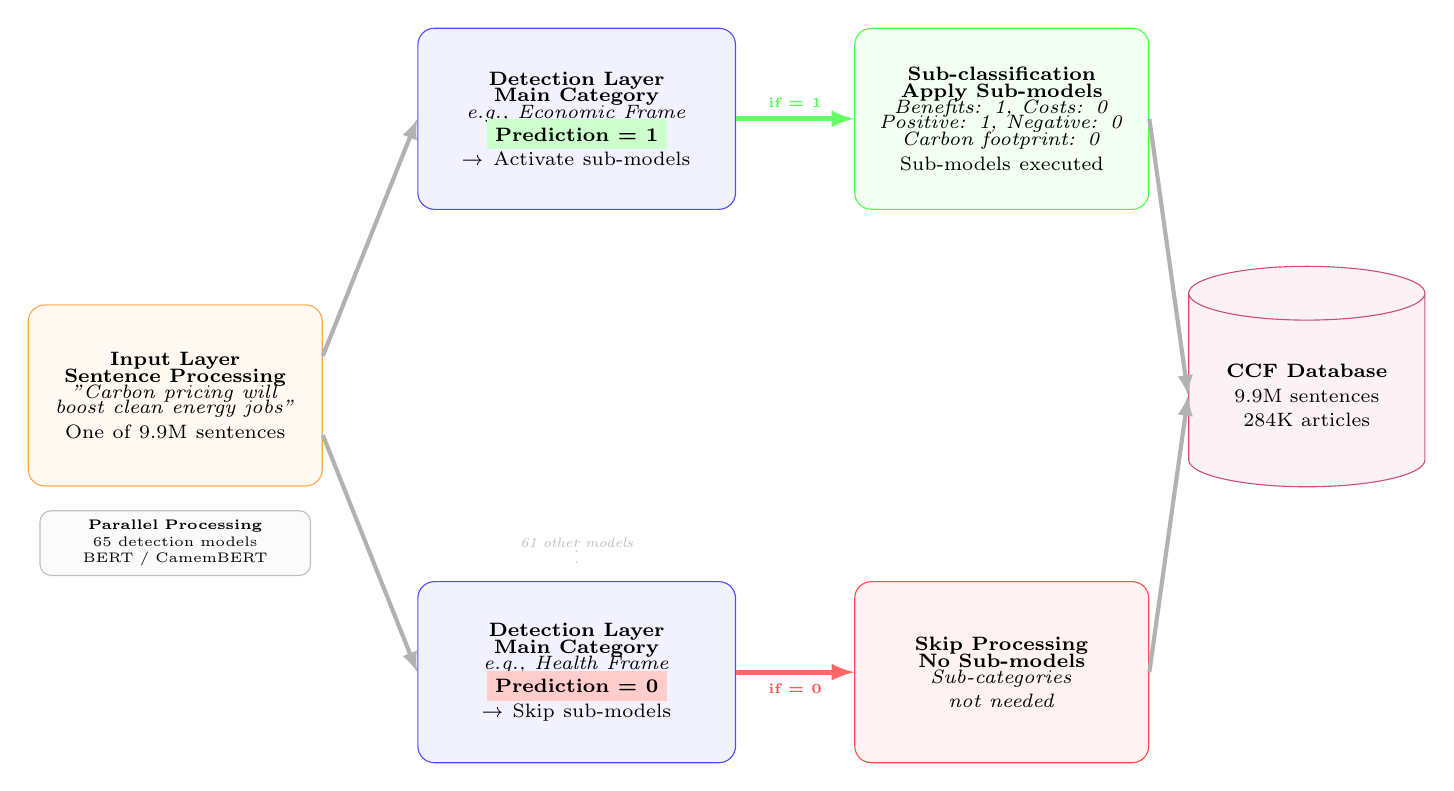
\begin{tikzpicture}[
    stage/.style={rectangle, rounded corners=6pt, minimum height=2.3cm, text width=3.8cm, align=center, font=\small},
    input/.style={stage, draw=orange!70, fill=orange!5, text width=3.5cm},
    detect/.style={stage, draw=blue!70, fill=blue!5, text width=3.8cm},
    process/.style={stage, draw=green!70, fill=green!5, text width=3.5cm},
    skip/.style={stage, draw=red!70, fill=red!5, text width=3.5cm},
    storage/.style={cylinder, draw=purple!70, fill=purple!5, shape border rotate=90, minimum height=2.8cm, minimum width=3cm, align=center, font=\small, aspect=0.3},
    arrow/.style={->, >=latex, line width=1.5pt, color=gray!60},
    yes/.style={arrow, color=green!60},
    no/.style={arrow, color=red!60},
    label/.style={font=\tiny\bfseries}
]

\node[input] (input) {
    \scriptsize\textbf{Input Layer}\\[-2pt]
    \scriptsize\textbf{Sentence Processing}\\[-2pt]
    \textit{\scriptsize "Carbon pricing will}\\[-2.5pt]
    \textit{\scriptsize boost clean energy jobs"}\\[-2pt]
    \scriptsize{One of \CCFsentApprox{}M sentences}
};

\node[detect, above right=1.2cm and 1.2cm of input] (detect_yes) {
    \scriptsize\textbf{Detection Layer}\\[-2pt]
    \scriptsize\textbf{Main Category}\\[-2pt]
    \textit{\scriptsize e.g., Economic Frame}\\[-2pt]
    \colorbox{green!20}{\scriptsize\textbf{Prediction = 1}}\\[-2pt]
    \scriptsize{→ Activate sub-models}
};

\node[detect, below right=1.2cm and 1.2cm of input] (detect_no) {
    \scriptsize\textbf{Detection Layer}\\[-2pt]
    \scriptsize\textbf{Main Category}\\[-2pt]
    \textit{\scriptsize e.g., Health Frame}\\[-2pt]
    \colorbox{red!20}{\scriptsize\textbf{Prediction = 0}}\\[-2pt]
    \scriptsize{→ Skip sub-models}
};

\node[process, right=1.5cm of detect_yes] (execute) {
    \scriptsize\textbf{Sub-classification}\\[-2pt]
    \scriptsize\textbf{Apply Sub-models}\\[-2pt]
    \textit{\scriptsize Benefits: 1, Costs: 0}\\[-2.5pt]
    \textit{\scriptsize Positive: 1, Negative: 0}\\[-2pt]
    \textit{\scriptsize Carbon footprint: 0}\\[-2pt]
    \scriptsize{Sub-models executed}
};

\node[skip, right=1.5cm of detect_no] (bypass) {
    \scriptsize\textbf{Skip Processing}\\[-2pt]
    \scriptsize\textbf{No Sub-models}\\[-2pt]
    \textit{\scriptsize Sub-categories}\\[-2.5pt]
    \textit{\scriptsize not needed}
};

\node[storage] (database) at ($(execute.east)!0.5!(bypass.east) + (2cm,0)$) {
    \scriptsize\textbf{CCF Database}\\[-2pt]
    \scriptsize \CCFsentApprox{}M sentences\\[-2.5pt]
    \scriptsize 284K articles
};

\draw[arrow] (input.15) -- (detect_yes.west);
\draw[arrow] (input.-15) -- (detect_no.west);
\draw[yes, line width=1.8pt] (detect_yes) -- node[above, label] {\textcolor{green!70}{if = 1}} (execute);
\draw[no, line width=1.8pt] (detect_no) -- node[below, label] {\textcolor{red!70}{if = 0}} (bypass);
\draw[arrow] (execute.east) -- (database.west);
\draw[arrow] (bypass.east) -- (database.west);

\node[below=0.3cm of input, draw=gray!50, fill=gray!3, rounded corners=4pt, text width=3.2cm, align=center, font=\tiny] {
    \textbf{Parallel Processing}\\
    65 detection models\\
    BERT / CamemBERT
};

\node[above=0.3cm of detect_no, font=\tiny\itshape, text=gray!50] {61 other models};
\node[above=0.1cm of detect_no, font=\tiny, text=gray!50] {$\vdots$};

\end{tikzpicture}
}
\caption{Hierarchical annotation pipeline. The system processes each sentence through detection models that determine whether corresponding sub-category models should be applied, enabling efficient annotation of the entire corpus.}
\label{fig:hierarchical_annotation}
\end{figure}

Once the per-category models had been finalised, all trained models were applied to annotate the complete CCF Database of \CCFsentApprox{}~million sentences across \CCFarticles{} articles. A hierarchical classification strategy was implemented that directly mirrored the annotation protocol's structure of primary categories and their associated sub-categories, as illustrated in Figure~\ref{fig:hierarchical_annotation}.

The hierarchical approach reflected the conceptual organisation of the annotation framework with eleven primary detection categories, each with specific sub-categories. The eight main frames (\emph{Economic}, \emph{Health}, \emph{Security}, \emph{Justice}, \emph{Political}, \emph{Scientific}, \emph{Environmental}, and \emph{Cultural Frame}) functioned as primary categories with their internal distinctions---for example, \emph{Economic Frame}, when positive (=1), triggered five economic sub-models (\emph{negative/positive economic impacts of climate change}, \emph{economic disadvantages/benefits of climate action}, \emph{carbon footprint of the economic sector}), while a negative detection (=0) bypassed these entirely.

Similarly, the three other primary categories followed this conditional logic: \emph{Actors/Messengers Detection} activated nine actor-type sub-models (\emph{Health Expert}, \emph{Economic Expert}, \emph{Security Expert}, \emph{Legal Expert}, \emph{Cultural Expert}, \emph{Natural Scientist}, \emph{Social Scientist}, \emph{Activist}, \emph{Public Official}), \emph{Event Detection} triggered eight event-type classifications (\emph{Extreme Weather Event}, \emph{Meeting/Conference}, \emph{Publication}, \emph{Election}, \emph{Policy Announcement}, \emph{Judiciary Decision}, \emph{Cultural Event}, \emph{Protest}), and \emph{Solutions Detection} applied two solution sub-categories (\emph{Mitigation Strategy}, \emph{Adaptation Strategy}). The deployment also processed standalone primary categories without hierarchical structure---\emph{Emotional Tone} (\emph{Positive Emotion}/\emph{Negative Emotion}/\emph{Neutral Emotion}), \emph{Geographic Focus} (\emph{Canadian Context}), \emph{Urgency/Alarmism}.

In addition to the custom-trained classification models, three pre-trained Named Entity Recognition (NER) models were employed, selected on the basis of empirical evaluation on the CCF data. A hybrid approach tailored to each language was implemented. For English texts, the publicly available \texttt{dslim/bert-base-NER}\ model (hosted on the Hugging Face Hub) was used for all three entity types: persons, organisations, and locations. For French texts, person entities were extracted with the spaCy \texttt{fr\_core\_news\_lg} pipeline, while organisations and locations were extracted with the \texttt{Jean-Baptiste/camembert-ner}\ model (also hosted on the Hugging Face Hub). This hybrid strategy was chosen to leverage the respective strengths of each model: spaCy's superior performance on French person names, and CamemBERT-NER's robust identification of French organisational and geographical entities. Per-language performance metrics for the three NER models are reported in Supplementary Table~S6.

\subsection{Phase 5: Database enrichment}
\label{subsec:database_enrichment}

The deployment described above produced the two original tables of the CCF Database (\texttt{CCF\_full\_data} and \texttt{CCF\_processed\_data}). The database was then further enriched with four additional tables and a complete index structure so that researchers could interrogate the corpus without rewriting the same article-level aggregations on every project. The enrichment procedure was deterministic and idempotent: it ran end-to-end from a freshly restored database dump, and each step (index provisioning, article-level aggregates, article-level entities, sentence embeddings, and reliability tiers) is described in detail below.

{\bfseries{Indexes.}} The first enrichment step provisioned twenty indexes on the two original tables: unique primary keys on \texttt{(doc\_id)} for \texttt{CCF\_full\_data} and \texttt{(doc\_id, sentence\_id)} for \texttt{CCF\_processed\_data}; routine B-trees on the columns researchers query most frequently (\texttt{date}, \texttt{media}, \texttt{language}); and partial B-trees on \texttt{doc\_id} restricted to the rows where one of the eleven primary detection flags is positive (\emph{economic\_frame}, \emph{health\_frame}, \emph{security\_frame}, \emph{justice\_frame}, \emph{political\_frame}, \emph{scientific\_frame}, \emph{environmental\_frame}, \emph{cultural\_frame}, \emph{messenger}, \emph{event}, \emph{solution}). The partial indexes accelerated the most common analytical workflow---retrieving the subset of articles or sentences in which a given frame is positive---without paying the storage cost of a full B-tree on each binary column.

{\bfseries{Article-level aggregates.}} The \texttt{CCF\_article\_aggregates} table was built with one row per \texttt{doc\_id}; for each of the 65 annotation categories, it stored the article-level proportion (\texttt{prop\_X}, in $[0, 1]$) of sentences positive for category $X$, computed as the sum of the binary flag divided by the article's sentence count. The table also recorded the article's sentence count overall and by language (\texttt{n\_sentences}, \texttt{n\_sentences\_en}, \texttt{n\_sentences\_fr}), the article's top frame (\texttt{top\_frame}, the main frame with the highest proportion in the article), the proportion of that frame (\texttt{top\_frame\_prop}), the Shannon entropy of the eight main-frame proportions (\texttt{entropy\_frames}, measuring how concentrated or diffuse the article's framing is), and the number of distinct messenger, event, and solution sub-categories present in the article (\texttt{n\_unique\_messenger\_subs}, \texttt{n\_unique\_event\_subs}, \texttt{n\_unique\_solution\_subs}). Sub-categories whose parent primary detection was negative were coalesced to zero, so a \texttt{prop\_X} reading of 0 unambiguously means \enquote{no sentence in this article is positive for category $X$}, regardless of whether the sub-category was hierarchically evaluated.

{\bfseries{Article-level named entities.}} The \texttt{CCF\_article\_entities} table consolidated the sentence-level Named Entity Recognition output (the \texttt{ner\_entities} JSON column in \texttt{CCF\_processed\_data}) into one row per article. Three JSONB arrays (\texttt{entities\_per}, \texttt{entities\_org}, \texttt{entities\_loc}) stored the deduplicated set of persons, organisations, and locations mentioned anywhere in the article; three counters (\texttt{n\_unique\_per}, \texttt{n\_unique\_org}, \texttt{n\_unique\_loc}) recorded their cardinalities; and three further counters reported how many sentences of the article contained at least one entity of each type. The presence of an entity in this rollup does not by itself disambiguate whether the entity is the speaker, the subject, or a passing reference; users wishing to recover speaker--statement attribution should combine the entity rollup with the sentence-level \texttt{messenger} family of annotations or with downstream attribution models that are out of scope for this database.

{\bfseries{Sentence embeddings.}} The \texttt{CCF\_sentence\_embeddings} table was populated, for every sentence in \texttt{CCF\_processed\_data} and for the title of every article (encoded as \texttt{sentence\_id} = 0), with the dense vector representation produced by the BAAI \texttt{bge-m3} multilingual encoder \autocite{chen_bge_2024}. \texttt{bge-m3} was selected for three reasons: (i)~it natively supports the 100+ languages relevant to bilingual Canadian coverage and is reported to perform competitively on French--English cross-lingual tasks; (ii)~it produces 1024-dimensional dense vectors that combine acceptable retrieval quality with manageable storage overhead; and (iii)~it has been stable and widely adopted since its January~2024 release, which is favourable for the long-term reproducibility expected of a published dataset. Vectors were L2-normalised at encoding time, so cosine similarity reduces to a dot product and can be queried directly through the \texttt{pgvector} \texttt{<=>} operator. Storage used the \texttt{halfvec(1024)} type ($2$~bytes per dimension, identical to the upstream \texttt{float16} representation), and an HNSW index on the cosine operator class was built to deliver sub-second approximate top-$k$ retrieval over the \CCFsentApprox{}~million-row table.

{\bfseries{Reliability tiers.}} The last enrichment step recorded, for each annotation category, a recommendation on how confidently it can be used in downstream analyses. The recommendation was summarised as a discrete \emph{reliability tier} derived from the two evaluation criteria reported in full in the \hyperref[sec:technical_validation]{Technical Validation section} below---the validation macro $F_1$ score against the gold standard, and the blind-phase Cohen's $\kappa$ between the expert annotator and the independent second coder. The \texttt{CCF\_reliability\_tiers} table was built as a 65-row lookup classifying each category into one of three tiers: Tier~A (\emph{research-grade}) required $F_1 \geq 0.80$ \emph{and} $\kappa \geq 0.60$; Tier~C (\emph{exploratory}) corresponded to $F_1 < 0.60$ \emph{or} $\kappa < 0.40$; Tier~B (\emph{use with caution}) captured everything in between. The table also flagged the categories affected by \emph{prevalence-induced reliability deflation}---that is, categories for which $F_1 \geq 0.70$ but $\kappa < 0.40$, where the chance-corrected agreement is depressed by very low prevalence rather than by systematic disagreement between coders \autocite{feinstein_high_1990, byrt_bias_1993}---and the two categories without an English model (annotated on French sentences only). Because the annotation tables store one \emph{column} per category while the tier table stores one \emph{row} per category, the two are not combined through a relational join: \texttt{CCF\_reliability\_tiers} is a lookup that tells the analyst \emph{which columns} of \texttt{CCF\_processed\_data} or \texttt{CCF\_article\_aggregates} to keep. Selecting the codes where \texttt{tier\_overall = 'A'} and restricting the analysis to the corresponding columns limits it to the 27~categories that the authors recommend without reservation; a worked example is given in the Usage Notes section, and the full tier assignment by language is provided in Supplementary Table~S10.

A diagram of the enriched database, together with the join paths that connect the six tables, appears in the Data Records section (Figure~\ref{fig:database_structure}). The complete enrichment procedure ran end-to-end in approximately 2.5~hours on a single Apple Mac~Studio with the M2~Ultra chip and 128~GB of unified memory.



\section{Data Records}
\label{sec:data_records}

Before working with any table of the deposit, users are advised to consult the \texttt{CCF\_reliability\_tiers} lookup described in this section: it assigns each of the 65 annotation categories an A/B/C reliability tier, and the authors recommend restricting substantive conclusions to Tier~A categories (27 of 65) unless the analysis explicitly accounts for the uncertainty of lower tiers. The database is versioned: new releases are published on Zenodo approximately every six months, as the CCF Observatory---the continuous extraction, annotation, and enrichment pipeline that now maintains the corpus---ingests newly published articles. The concept DOIs (\CCFsqldoiConcept{} for the PostgreSQL edition, \CCFparquetdoiConcept{} for the Parquet mirror) always resolve to the latest release, while version DOIs remain permanently resolvable so that any analysis can be reproduced against the exact release it used. This paper describes version~\CCFversion{}.

\subsection{Overview of the deposit}

\begin{figure}[H]
\centering
\resizebox{0.92\textwidth}{!}{%
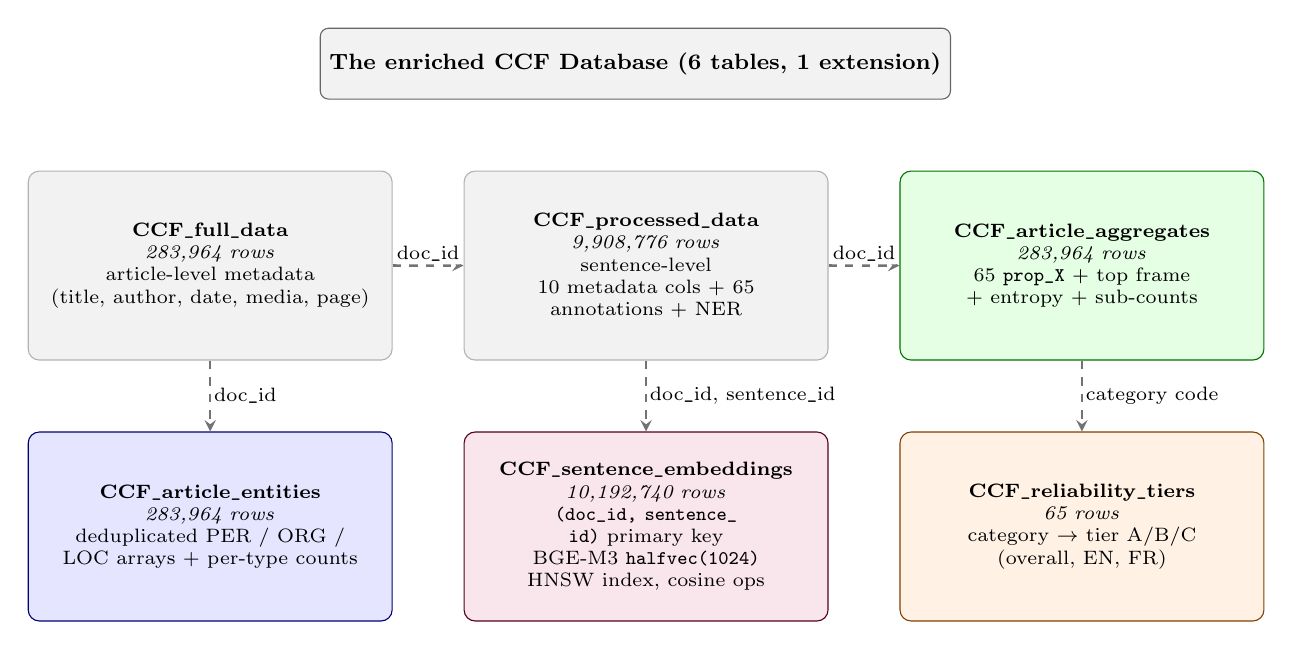
\begin{tikzpicture}[
    node distance=0.9cm and 0.9cm,
    header/.style={rectangle, draw=black!60, rounded corners=3pt, fill=gray!10, minimum width=7cm, minimum height=0.9cm, align=center, font=\footnotesize\bfseries},
    table/.style={rectangle, draw=black!50, rounded corners=4pt, minimum width=4.4cm, minimum height=2.4cm, align=center, font=\scriptsize, text width=4.2cm, inner sep=6pt},
    orig/.style={table, fill=gray!10, draw=gray!60},
    aggr/.style={table, fill=green!10, draw=green!45!black},
    ent/.style={table,  fill=blue!10,  draw=blue!45!black},
    rel/.style={table,  fill=orange!10, draw=orange!50!black},
    embed/.style={table, fill=purple!10, draw=purple!45!black},
    arrow/.style={->, >=stealth, thick, draw=black!55, dashed},
    edgelbl/.style={font=\scriptsize, fill=white, inner sep=1pt, rounded corners=1pt},
]
\node[header] (head) {The enriched CCF Database (6 tables, 1 extension)};
\node[orig, below=of head, xshift=-5.4cm] (full)  {\textbf{CCF\_full\_data}\\\textit{\CCFarticles{} rows}\\article-level metadata\\(title, author, date, media, page)};
\node[orig, right=of full] (proc) {\textbf{CCF\_processed\_data}\\\textit{\CCFsentences{} rows}\\sentence-level\\10 metadata cols + 65 annotations + NER};
\node[aggr, right=of proc] (aggr) {\textbf{CCF\_article\_aggregates}\\\textit{\CCFarticles{} rows}\\65 \texttt{prop\_X} + top frame + entropy + sub-counts};
\node[ent,  below=of full]  (ent)  {\textbf{CCF\_article\_entities}\\\textit{\CCFarticles{} rows}\\deduplicated PER / ORG / LOC arrays + per-type counts};
\node[rel,  below=of aggr]  (rel)  {\textbf{CCF\_reliability\_tiers}\\\textit{65 rows}\\category $\rightarrow$ tier A/B/C\\(overall, EN, FR)};
\node[embed,below=of proc]  (embed){\textbf{CCF\_sentence\_embeddings}\\\textit{\CCFembeddings{} rows}\\\texttt{(doc\_id, sentence\_id)} primary key\\BGE-M3 \texttt{halfvec(1024)}\\HNSW index, cosine ops};

% Horizontal joins on the top row.
\draw[arrow] (full.east)  -- node[edgelbl, above] {doc\_id} (proc.west);
\draw[arrow] (proc.east)  -- node[edgelbl, above] {doc\_id} (aggr.west);
% Vertical joins. Anchored at distinct horizontal positions on the
% top row so the labels do not overlap.
\draw[arrow] (full.south) -- node[edgelbl, right] {doc\_id} (ent.north);
\draw[arrow] (proc.south) -- node[edgelbl, right] {doc\_id, sentence\_id} (embed.north);
\draw[arrow] (aggr.south) -- node[edgelbl, right] {category code} (rel.north);
\end{tikzpicture}
}%
\caption{Schema of the enriched CCF Database. Dashed arrows indicate the join paths between tables; column types and full schemas are documented in Supplementary Table~S12. \texttt{CCF\_full\_data} and \texttt{CCF\_processed\_data} are the original sentence-level resource; the three coloured groups are the article-level rollups (green), the reliability lookup (orange), and the embedding table (purple).}
\label{fig:database_structure}
\end{figure}

The CCF Database is deposited on Zenodo under a CC-BY~4.0 licence in two complementary editions sharing identical schemas. The canonical PostgreSQL edition (DOI \CCFsqldoi{}~\autocite{lemor_ccf_database_2026}) ships as a single tarball (\texttt{CCF\_Database.tar}, $\approx$~\CCFsqlsize{}~GB) wrapping a \texttt{pg\_dump} \emph{directory} archive of the six relational tables together with all B-tree, partial, and HNSW indexes; restoration requires PostgreSQL~16 or~17 with the \texttt{pgvector} extension ($\geq$~0.8.2 for \texttt{halfvec} support) and the deposit's README provides the exact three-line restore command (\texttt{tar -xf}, \texttt{createdb}, \texttt{pg\_restore -j 8}). A sister column-oriented Apache Parquet mirror (DOI \CCFparquetdoi{}~\autocite{lemor_ccf_database_parquet_2026}, one ZSTD-compressed file per table, $\approx$~\CCFparquetsize{}~GB) is provided for users without a PostgreSQL backend; the \texttt{halfvec(1024)} embedding column is materialised as a 1024-element \texttt{LIST<FLOAT>} and the JSONB entity arrays are serialised as UTF-8 JSON strings, so each Parquet file can be read directly with \texttt{pandas}, \texttt{polars}, R/\texttt{arrow}, DuckDB, or Spark. The companion code and documentation---the full annotation pipeline (\texttt{Scripts/Annotation/}), the enrichment and export scripts (\texttt{Scripts/Database\_creation/}), and the canonical CSVs underlying the supplementary tables (\texttt{Database/Training\_data/})---are archived in a dedicated, versioned Zenodo deposit (DOI \CCFcodedoi{}~\autocite{lemor_ccf_code_2026}) and, for convenience, also bundled with both data editions as \texttt{ccf\_code\_and\_paper.tar.gz}; a development mirror is maintained on GitHub (\texttt{antoinelemor/CCF-canadian-climate-framing}, referenced in the Code Availability statement).

Because Canadian newspaper articles are protected by copyright, the deposit does not redistribute the raw sentence text or full article bodies of the corpus at large. What is shared is everything else: article-level metadata (titles, authors, publication dates, newspapers, page numbers), sentence-level identifiers, the 65 binary annotations, the named-entity extractions, the article-level aggregates and entity rollups, the per-category reliability tiers, and the BGE-M3 sentence embeddings. One deliberate, clearly bounded exception is made so that the single-coder training protocol and the gold standard can be independently audited: the code and documentation deposit releases the expert-coded sentences themselves---the $\sim$4{,}000 training sentences (\texttt{Database/Training\_data/manual\_annotations\_JSONL/Annotated\_sentences.jsonl}, together with the per-category train/validation splits under \texttt{annotation\_bases/}) and the 1{,}000-sentence double-coded gold standard (\texttt{blind\_verification.jsonl} and \texttt{consensus\_gold\_standard.jsonl}). These files contain short excerpts of two sentences each, quoted for the purpose of research and validation with full bibliographic attribution through the corpus metadata; this reproduction of brief extracts falls under the fair-dealing exception for research and private study of the Canadian \emph{Copyright Act} (s.~29) and does not substitute for the original works. Each article in the corpus is identified by its bibliographic coordinates (\texttt{media}, \texttt{date}, \texttt{title}, \texttt{author}, \texttt{page\_number}), which is the standard bibliographic reference for Canadian newspapers and is sufficient for any researcher with institutional access to Factiva, Eureka.cc, or ProQuest Canadian Major Dailies to retrieve the original text. No DOIs exist for the historical articles covered by the corpus.

The database is organised around two original tables produced by the annotation pipeline (\texttt{CCF\_full\_data}, \texttt{CCF\_processed\_data}) and four enrichment tables that pre-compute the queries most frequently issued by analysts (article-level aggregates, article-level entities, reliability tiers, sentence embeddings). The schema is summarised in Table~\ref{tab:tables_overview} and depicted graphically in Figure~\ref{fig:database_structure}; the join paths in that diagram point to the recommended foreign keys whenever a query needs to combine two tables.

\begin{table}[h!]
\centering
\caption{Overview of the six tables in the deposited CCF Database. The \texttt{pgvector} extension underpins the \texttt{CCF\_sentence\_embeddings} table.}
\label{tab:tables_overview}
\footnotesize
\renewcommand{\arraystretch}{1.2}
\begin{tabularx}{\textwidth}{>{\ttfamily}p{4.2cm} r >{\raggedright\arraybackslash}p{2.6cm} X}
\toprule
\textnormal{\textbf{Table}} & \textbf{Rows} & \textbf{Granularity} & \textbf{What it stores} \\
\midrule
CCF\_full\_data            & \CCFarticles{}     & Article  & Bibliographic metadata for every article in the corpus. \\
CCF\_processed\_data       & \CCFsentences{} & Sentence & The 65 sentence-level binary annotations and the per-sentence NER output. \\
CCF\_article\_aggregates   & \CCFarticles{}     & Article  & Per-article proportions, top frame, framing entropy and sub-category counts. \\
CCF\_article\_entities     & \CCFarticles{}     & Article  & Deduplicated JSONB arrays of PER / ORG / LOC mentions, with per-type cardinalities and per-type sentence counts. \\
CCF\_reliability\_tiers    & 65            & Category & Per-category reliability tier (A / B / C) with the underlying $F_1$ and $\kappa$ values. \\
CCF\_sentence\_embeddings  & \CCFembeddings{} & Sentence + title & L2-normalised BGE-M3 1024-dimensional vectors, queryable through \texttt{pgvector}. \\
\bottomrule
\end{tabularx}
\end{table}

\subsection{\texttt{CCF\_full\_data} -- article-level metadata}
\label{subsec:data_full}

This table is the canonical inventory of articles in the corpus and the natural entry point for any analysis that operates at the article level. Each of its \CCFarticles{} rows describes one unique article and is uniquely keyed by \texttt{doc\_id}; every other table in the database joins back to \texttt{CCF\_full\_data} through this identifier. The columns are summarised in Table~\ref{tab:cols_full_data}.

\begin{table}[h!]
\centering
\caption{Columns of \texttt{CCF\_full\_data}.}
\label{tab:cols_full_data}
\footnotesize
\renewcommand{\arraystretch}{1.2}
\begin{tabularx}{\textwidth}{>{\ttfamily}p{2.6cm} >{\ttfamily}p{2.6cm} X}
\toprule
\textnormal{\textbf{Column}} & \textnormal{\textbf{Type}} & \textbf{Definition} \\
\midrule
doc\_id        & BIGINT (PK)   & Unique article identifier; foreign-key target for every other table. \\
news\_type     & TEXT          & Editorial category: news, opinion, editorial, etc. \\
title          & TEXT          & Article headline. \\
author         & TEXT          & Author byline when available. \\
media          & TEXT          & Newspaper name. \\
words\_count   & BIGINT        & Total word count of the article. \\
date           & DATE          & Publication date. \\
language       & TEXT          & ``EN'' or ``FR''. \\
page\_number   & TEXT          & Print page (free text, e.g.\ ``A1'' or ``B3''). \\
\bottomrule
\end{tabularx}
\end{table}

\subsection{\texttt{CCF\_processed\_data} -- sentence-level annotations}
\label{subsec:data_processed}

\begin{table}[b!]
\centering
\caption{Structural columns of \texttt{CCF\_processed\_data}. The 65 binary annotation columns are defined in Supplementary Table~S3.}
\label{tab:cols_processed_data}
\footnotesize
\renewcommand{\arraystretch}{1.2}
\begin{tabularx}{\textwidth}{>{\ttfamily}p{2.6cm} >{\ttfamily}p{2.6cm} X}
\toprule
\textnormal{\textbf{Column}} & \textnormal{\textbf{Type}} & \textbf{Definition} \\
\midrule
doc\_id         & BIGINT       & Foreign key to \texttt{CCF\_full\_data}. \\
sentence\_id    & BIGINT       & Position of the sentence within its article (starting at~1). \texttt{sentence\_id} = 0 is reserved for the article title in the embeddings table. \\
\textnormal{(metadata)} & \textnormal{various} & Ten metadata columns duplicated from \texttt{CCF\_full\_data} for query convenience: \texttt{news\_type}, \texttt{title}, \texttt{author}, \texttt{media}, \texttt{words\_count}, \texttt{date}, \texttt{language}, \texttt{page\_number}. \\
\textnormal{65 annotation columns} & \textnormal{INTEGER (0/1, nullable)} & One binary flag per category from Supplementary Table~S3. Sub-categories are NULL when the parent primary detection is negative. \\
ner\_entities   & TEXT (JSON)  & Per-sentence NER output in the format \texttt{\{"PER": [..], "ORG": [..], "LOC": [..]\}}. \\
\bottomrule
\end{tabularx}
\end{table}

This is the workhorse table of the database. It contains one row per two-sentence analytical unit, so \CCFsentences{} rows in total, and every annotation produced by the machine-learning pipeline lives here. The same ten metadata columns as \texttt{CCF\_full\_data} are denormalised on every row so that sentence-level queries can run without joining back to the article table whenever the analyst only needs the date, the newspaper, or the language. On top of that, the table stores the 65 binary annotation columns named exactly as in Supplementary Table~S3, and one JSON column (\texttt{ner\_entities}) holding the per-sentence Named Entity Recognition output. Sub-category columns are NULL when their parent primary detection is negative; researchers who want to treat ``absent'' as equivalent to ``not detected'' should coalesce NULL to zero, which is exactly the convention adopted by \texttt{CCF\_article\_aggregates}. The structural columns are summarised in Table~\ref{tab:cols_processed_data}.

\subsection{\texttt{CCF\_article\_aggregates} -- article-level rollup}
\label{subsec:data_aggregates}

\texttt{CCF\_article\_aggregates} is the recommended starting point for most article-level analyses---bearing in mind the general recommendation that opens this section: its 65 \texttt{prop\_*} columns inherit the reliability of the underlying sentence-level classifiers, so analyses should prioritise the columns whose category is Tier~A in \texttt{CCF\_reliability\_tiers}. It collapses the \CCFsentApprox{}~million sentence-level rows into one row per article (\CCFarticles{} rows) and pre-computes the quantities that almost every project needs: the proportion of sentences positive for each of the 65 categories, the top frame, a measure of how concentrated or diffuse the framing of the article is, and the number of distinct sub-categories activated. Because these aggregates are computed once at enrichment time and indexed, a sentence-level \texttt{GROUP BY} on the \CCFsentApprox{}-million-row sentence table is rarely necessary once the aggregates are available. The columns are summarised in Table~\ref{tab:cols_article_aggregates}.

\begin{table}[h!]
\centering
\caption{Columns of \texttt{CCF\_article\_aggregates}.}
\label{tab:cols_article_aggregates}
\footnotesize
\renewcommand{\arraystretch}{1.2}
\begin{tabularx}{\textwidth}{>{\ttfamily}p{3.4cm} >{\ttfamily}p{2.6cm} X}
\toprule
\textnormal{\textbf{Column}} & \textnormal{\textbf{Type}} & \textbf{Definition} \\
\midrule
doc\_id         & BIGINT (PK)   & Foreign key to \texttt{CCF\_full\_data}. \\
n\_sentences    & INTEGER       & Total number of two-sentence analytical units in the article. \\
n\_sentences\_en, n\_sentences\_fr & INTEGER & Same count restricted to English / French sentences. \\
\textnormal{65 \texttt{prop\_X} columns} & \textnormal{DOUBLE PRECISION (\([0,1]\))} & Article-level proportion of sentences positive for category $X$. Sub-categories with a negative parent detection are coalesced to zero. \\
top\_frame      & TEXT             & Main frame with the highest \texttt{prop\_X}; NULL when no frame is positive. \\
top\_frame\_prop & DOUBLE PRECISION & Proportion of the top frame in the article. \\
entropy\_frames      & DOUBLE PRECISION & Shannon entropy (natural base) of the eight main-frame proportions; 0 when no main frame is positive. \\
n\_unique\_messenger\_subs & SMALLINT & Number of distinct messenger sub-categories present in the article (0--9). \\
n\_unique\_event\_subs     & SMALLINT & Same for event sub-categories (0--8). \\
n\_unique\_solution\_subs  & SMALLINT & Same for solution sub-categories (0--2). \\
\bottomrule
\end{tabularx}
\end{table}

\subsection{\texttt{CCF\_article\_entities} -- article-level named-entity rollup}
\label{subsec:data_entities}

\texttt{CCF\_article\_entities} consolidates the sentence-level Named Entity Recognition output (the \texttt{ner\_entities} JSON column in \texttt{CCF\_processed\_data}) into one row per article. The table is designed to answer the recurring analytical question \emph{which entities does an article mention?} without forcing the analyst to parse the JSON for every sentence. It contains \CCFarticles{} rows and its structure is summarised in Table~\ref{tab:cols_article_entities}.

\begin{table}[h!]
\centering
\caption{Columns of \texttt{CCF\_article\_entities}.}
\label{tab:cols_article_entities}
\footnotesize
\renewcommand{\arraystretch}{1.2}
\begin{tabularx}{\textwidth}{>{\ttfamily}p{3.4cm} >{\ttfamily}p{2.6cm} X}
\toprule
\textnormal{\textbf{Column}} & \textnormal{\textbf{Type}} & \textbf{Definition} \\
\midrule
doc\_id          & BIGINT (PK)   & Foreign key to \texttt{CCF\_full\_data}. \\
entities\_per    & JSONB         & Deduplicated array of persons mentioned in the article. \\
entities\_org    & JSONB         & Deduplicated array of organisations. \\
entities\_loc    & JSONB         & Deduplicated array of locations. \\
n\_unique\_per, n\_unique\_org, n\_unique\_loc & INTEGER & Cardinalities of the three arrays above. \\
n\_sentences\_with\_per, n\_sentences\_with\_org, n\_sentences\_with\_loc & INTEGER & Number of sentences in the article that mention at least one entity of the corresponding type. \\
\bottomrule
\end{tabularx}
\end{table}

\subsection{\texttt{CCF\_reliability\_tiers} -- per-category quality lookup}
\label{subsec:data_reliability_tiers}

\texttt{CCF\_reliability\_tiers} provides a single-row-per-category recommendation on how confidently each of the 65 annotation categories may be used in downstream analyses. The tier assignment combines validation $F_1$ and blind-phase Cohen's $\kappa$ following the rules defined in Section~\ref{subsec:database_enrichment}; the underlying metrics and flags are kept in the same row so that researchers can refine the tier rule for their own use case if they wish. This table is a \emph{lookup}, not a join target: annotation categories appear as columns (not rows) in \texttt{CCF\_processed\_data} and \texttt{CCF\_article\_aggregates}, so the tier table is used to decide \emph{which columns} to retain---select the \texttt{code} values where \texttt{tier\_overall = 'A'} and restrict the analysis to those 27 columns (worked example in the Usage Notes). Columns are listed in Table~\ref{tab:cols_reliability_tiers}.

\begin{table}[h!]
\centering
\caption{Columns of \texttt{CCF\_reliability\_tiers}.}
\label{tab:cols_reliability_tiers}
\footnotesize
\renewcommand{\arraystretch}{1.2}
\begin{tabularx}{\textwidth}{>{\ttfamily}p{3.4cm} >{\ttfamily}p{2.6cm} X}
\toprule
\textnormal{\textbf{Column}} & \textnormal{\textbf{Type}} & \textbf{Definition} \\
\midrule
number          & SMALLINT (PK)  & Sequential index of the 65 deployed categories, in canonical framework order. Note that Supplementary Table~S3 enumerates all 67 \emph{candidate} categories (including the two excluded ones) and therefore numbers differently: categories should always be matched on \texttt{code}, never on \texttt{number}. S3 reports each category's \texttt{code} to make this crosswalk unambiguous. \\
category        & TEXT           & Readable category name. \\
code            & TEXT (UNIQUE)  & Column code as used in \texttt{CCF\_processed\_data}. \\
tier\_overall   & CHAR(1)        & Tier on the combined corpus: ``A'', ``B'', or ``C''. \\
tier\_en        & CHAR(1)        & Tier on the English subset. \\
tier\_fr        & CHAR(1)        & Tier on the French subset. \\
paradox\_kappa  & BOOLEAN        & True if the category exhibits prevalence-induced reliability deflation ($F_1 \geq 0.70$ and $\kappa < 0.40$). \\
exclusion\_reason & TEXT         & ``insufficient\_training\_data'' for the two categories that could not be trained, NULL otherwise. \\
f1\_macro\_all, f1\_macro\_en, f1\_macro\_fr & DOUBLE PRECISION & Validation macro $F_1$ score on the gold standard, overall and per language. \\
support\_all, support\_en, support\_fr & INTEGER & Number of positive (class~1) validation examples. \\
cohens\_kappa\_blind\_phase, gwet\_ac1\_blind\_phase, krippendorff\_alpha\_blind\_phase & DOUBLE PRECISION & Inter-coder agreement on the blind phase (sentences 601--1000). \\
n\_blind\_phase & INTEGER         & Sentence count of the blind phase. \\
prev\_coder1\_full, prev\_coder2\_full & DOUBLE PRECISION & Prevalence (proportion of positives) per coder on the full 1{,}000-sentence sample. \\
\bottomrule
\end{tabularx}
\end{table}

\subsection{\texttt{CCF\_sentence\_embeddings} -- dense vector representations}
\label{subsec:data_embeddings}

\texttt{CCF\_sentence\_embeddings} enables semantic retrieval and similarity-based analyses across the whole corpus. It holds one row per sentence (and one extra row per article title, encoded with \texttt{sentence\_id} = 0), for a total of \CCFembeddings{} rows. Each row stores a 1024-dimensional BAAI/bge-m3 vector that is L2-normalised at encoding time, so cosine similarity reduces to a dot product and can be queried directly through the \texttt{pgvector} \texttt{<=>} operator. Storage uses the \texttt{halfvec(1024)} type (2 bytes per dimension, identical to the upstream \texttt{float16} representation), and an HNSW index on the cosine operator class delivers sub-second approximate top-$k$ retrieval over the full table. Columns are summarised in Table~\ref{tab:cols_sentence_embeddings}.

\begin{table}[h!]
\centering
\caption{Columns of \texttt{CCF\_sentence\_embeddings}.}
\label{tab:cols_sentence_embeddings}
\footnotesize
\renewcommand{\arraystretch}{1.2}
\begin{tabularx}{\textwidth}{>{\ttfamily}p{3.4cm} >{\ttfamily}p{3.0cm} X}
\toprule
\textnormal{\textbf{Column}} & \textnormal{\textbf{Type}} & \textbf{Definition} \\
\midrule
doc\_id      & BIGINT (PK, with sentence\_id) & Foreign key to \texttt{CCF\_full\_data}. \\
sentence\_id & INTEGER (PK)                   & Sentence position within the article. \texttt{sentence\_id} = 0 is reserved for the article title. \\
embedding    & \texttt{halfvec(1024)}         & L2-normalised BGE-M3 vector. Cosine distance is computed via the \texttt{pgvector} \texttt{<=>} operator; an HNSW index on the cosine operator class is provisioned by the enrichment pipeline. \\
\bottomrule
\end{tabularx}
\end{table}

The complete data dictionary, including every column type and the full set of join paths, is provided in Supplementary Table~S12.

\section{Data Overview}
\label{sec:data_overview}

This section consolidates three reproducible summaries of the deposited CCF Database. Every figure and table is generated by the script \texttt{Results/Scripts/3\_data\_overview.py}, which pulls the underlying numbers directly from the deposited PostgreSQL tables: no manual transcription is involved, and re-running the script regenerates the artefacts byte-for-byte.


\begin{table}[p]
\centering
\caption{Article-level descriptive statistics of the deposited CCF Database. Mean share is the average per-article proportion of sentences positive for the category; the top-frame column reports the percentage of articles for which the frame has the highest share among the eight frames. Computed from \texttt{CCF\_full\_data}, \texttt{CCF\_processed\_data}, and \texttt{CCF\_article\_aggregates}.}
\label{tab:data_overview_descriptives}
\medbreak
{\scriptsize\renewcommand{\arraystretch}{1.05}
\input{../Results/Outputs/Tables/table_data_overview_descriptives.tex}}
\end{table}

\begin{figure}[p]
\centering
\includegraphics[width=\textwidth,height=0.22\textheight,keepaspectratio]{Figures/data_overview_frames_lines.png}
\caption{Mean per-article share of each main frame, year by year, 1980--\CCFyearlast{}. Each point is the mean of the corresponding \texttt{prop\_X} column of \texttt{CCF\_article\_aggregates} across the articles published in that year, joined with \texttt{CCF\_full\_data} on \texttt{doc\_id}. The pre-1988 portion of the curve is computed on fewer than fifty articles per year.}
\label{fig:data_overview_frames_lines}
\end{figure}

\begin{table}[p]
\centering
\caption{Ten most frequently mentioned entities of each type in the deposited CCF Database. ``Articles'' is the number of articles in which the entity appears at least once. Computed from the JSONB arrays of \texttt{CCF\_article\_entities} (\texttt{entities\_per}, \texttt{entities\_org}, \texttt{entities\_loc}).}
\label{tab:data_overview_entities}
\medbreak
{\scriptsize\renewcommand{\arraystretch}{1.05}\setlength{\tabcolsep}{5pt}
\input{../Results/Outputs/Tables/table_data_overview_entities.tex}}
\end{table}


{\bfseries{Article-level descriptive statistics.}} Table~\ref{tab:data_overview_descriptives} reports the corpus size (article count, two-sentence analytical units, and per-article word statistics) computed on \texttt{CCF\_full\_data} and \texttt{CCF\_processed\_data}, and the mean per-article share of sentences positive for each annotation category, computed on the \texttt{prop\_X} columns of \texttt{CCF\_article\_aggregates}. The left block lists the eight frames together with the percentage of articles for which each frame is the \texttt{top\_frame}; the right block lists the primary categories (messenger, event, solution, Canadian context, urgency) and the three tones.

{\bfseries{Temporal coverage of the main frames.}} Figure~\ref{fig:data_overview_frames_lines} plots, for every calendar year between 1980 and \CCFyearlast{}, the mean of each \texttt{prop\_X} main-frame column of \texttt{CCF\_article\_aggregates}, grouped by the year extracted from \texttt{CCF\_full\_data.date}. No smoothing or regression is applied; each point is a yearly mean. The earliest years of the corpus carry very few articles---fewer than fifty per year before 1988 and fewer than five hundred per year before 1990---so the pre-1988 portion of the curve is computed on small samples and should be read with that caveat.

{\bfseries{Named-entity coverage.}} Table~\ref{tab:data_overview_entities} reports the ten most frequently mentioned entities of each NER type. Entities are extracted from the JSONB arrays \texttt{entities\_per}, \texttt{entities\_org}, and \texttt{entities\_loc} of \texttt{CCF\_article\_entities}, expanded with \texttt{jsonb\_array\_elements\_text}, filtered to remove pure punctuation and one-character tokens, and counted in articles---an entity is therefore counted once per article regardless of how many sentences mention it. Variants such as \emph{Trudeau} vs.\ \emph{Justin Trudeau} are kept separate because the underlying NER pipeline emits them as distinct strings; analysts who need canonicalised entities can apply their own resolution step on top of these arrays.

\clearpage
\section{Technical Validation}
\label{sec:technical_validation}

Technical validation of the CCF database and the trained models proceeded in three steps. First, a stratified validation set was constructed in line with established best practices for multi-label classification. Second, an expert annotator in climate change politics produced the reference annotations that define the gold standard used for all model evaluation. Third, an independent second annotator replicated the coding following a structured protocol comprising a training phase (sentences 1–600) and a blind coding phase (sentences 601–1000), enabling assessment of inter-coder reliability. The 1{,}000-sentence gold standard is strictly disjoint from the 4{,}000-sentence training/validation pool used in Phase~3. We explicitly excluded all sentence identifiers present in the training data before drawing the stratified sample, so that no test sentence was ever seen by a trained model at training time.

\subsection{Construction of the stratified validation set}

The validation set comprised 1,000 sentences (500 per language) extracted from the fully annotated database using a root-inverse probability weighting scheme combined with strict structural constraints. Each candidate sentence $i$ received a sampling weight
\begin{equation}
    w_i \;\propto\; \sum_{j \in C(i)} \frac{1}{\sqrt{f_j}},
\end{equation}
where $C(i)$ denotes the set of categories that are positive for sentence $i$ and $f_j$ denotes the corpus-wide prevalence of category $j$. The square root in the denominator deliberately moderated the influence of extremely rare categories, while still privileging them over common ones. Concretely, a sentence annotated with both \textit{Economic Frame} (15.4\% prevalence in the corpus) and \textit{Loss of Indigenous Practices} (0.28\% prevalence) received a weight of
\begin{equation*}
    \frac{1}{\sqrt{0.154}} + \frac{1}{\sqrt{0.0028}} \;=\; 2.55 + 18.90 \;=\; 21.45,
\end{equation*}
which was roughly eight times the weight of a sentence containing only \textit{Economic Frame}, and ensured that under-represented categories nevertheless reached the validation set.

Two structural constraints were then applied on top of this weighted draw. First, a floor of 40 positive examples per category was targeted at sampling time---counted on the \emph{model-predicted} labels, since sampling necessarily precedes the expert coding of the gold standard---so that each category would enter the validation set with as much statistical support as its corpus prevalence allowed. This target could not always be met for rare categories, and even where 40 predicted positives were drawn, the number of \emph{expert-confirmed} positives can be substantially lower: the effective support ranges from 2 (\textit{Disruption of military operations}, whose corpus prevalence is on the order of $10^{-5}$) to several hundred, and 23 of the 65 categories fall below 40 confirmed positives. The per-category support is reported in Supplementary Table~S7 so that readers can weigh each per-category estimate accordingly. Second, a 35\% maximum allocation per category was imposed to prevent any single prevalent category from monopolising the validation set; without this ceiling, \textit{Actors/Messengers Detection} alone, present in 48.8\% of database sentences, could plausibly have dominated the entire sample and left insufficient space for the rarer categories.


\begin{figure}[b!]
\centering
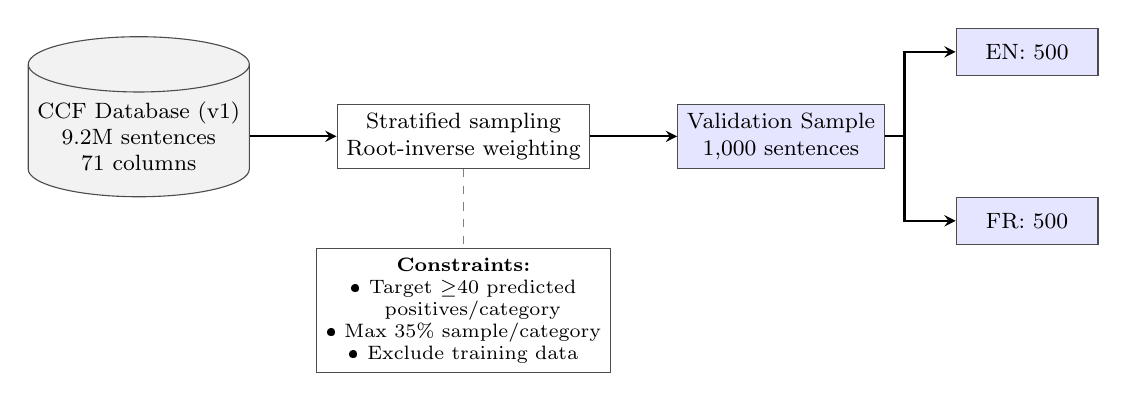
\begin{tikzpicture}[
    box/.style={rectangle, draw=black!70, fill=white, minimum width=2.2cm, minimum height=0.65cm, align=center, font=\footnotesize},
    database/.style={cylinder, draw=black!70, fill=gray!10, minimum width=2.4cm, minimum height=1cm, align=center, shape border rotate=90, aspect=0.25, font=\footnotesize},
    sample/.style={rectangle, draw=black!70, fill=blue!10, minimum width=1.8cm, minimum height=0.6cm, align=center, font=\footnotesize},
    arrow/.style={->, >=stealth, thick},
    node distance=1.1cm
]

\node[database] (db) at (-3.2,0) {\footnotesize CCF Database (v1)\\\footnotesize 9.2M sentences\\\footnotesize 71 columns};
\node[box, right=of db] (sampling) {\footnotesize Stratified sampling\\\footnotesize Root-inverse weighting};
\draw[arrow] (db.east) -- (sampling.west);
\node[sample, right=of sampling] (val) {\footnotesize Validation Sample\\\footnotesize 1,000 sentences};
\draw[arrow] (sampling.east) -- (val.west);
\node[sample, above right=0.35cm and 0.9cm of val] (en) {\footnotesize EN: 500};
\node[sample, below right=0.35cm and 0.9cm of val] (fr) {\footnotesize FR: 500};
\draw[arrow] (val.east) -- ++(0.25,0) |- (en.west);
\draw[arrow] (val.east) -- ++(0.25,0) |- (fr.west);
\node[box, below=1cm of sampling, text width=3.5cm, font=\scriptsize] (constraints) {\textbf{Constraints:}\\• Target $\geq$40 predicted\\\hphantom{• }positives/category\\• Max 35\% sample/category\\• Exclude training data};
\draw[dashed, gray] (sampling.south) -- (constraints.north);

\end{tikzpicture}
\vspace{0.15cm}
\caption{Stratified sampling procedure for final validation. Root-inverse probability weighting ensures balanced representation across all 65 annotation categories.}
\label{fig:validation_sampling}
\end{figure}

\subsection{Expert gold-standard annotation and model performance}

All 1,000 sentences in the validation set were manually annotated by an expert annotator specialising in climate change politics. These expert annotations defined the gold standard against which all model performance metrics reported in this section were computed.

Model performance against the gold standard is summarised through two complementary quantities, both reproducible from the deposited per-category metrics (\texttt{Database/Training\_data/final\_annotation\_metrics\_normalized.csv}, Supplementary Table~S7). The \emph{pooled} macro F1 aggregates the predictions of all 65 categories over the 1{,}000 gold-standard sentences into a single confusion matrix before computing the score: it reaches 0.866 overall (0.869 for English, 0.864 for French) and measures the quality of the annotation layer as a whole, weighting every annotation decision equally. The \emph{mean per-category} macro F1---the unweighted average of the 65 per-category macro F1 scores, i.e.\ the same aggregation as the training-phase figure of 0.826 reported in Phase~3---is 0.773. The like-for-like comparison is therefore 0.826 in training versus 0.773 on the gold standard: the ordinary out-of-sample decrease expected when models face an independent, disjoint sample, concentrated in the low-support categories whose estimates are noisiest. Two design features of the validation set should be kept in mind when reading the per-category values: the sampling deliberately over-represents sentences positive for low-prevalence categories (the root-inverse weighting above), which are precisely the categories targeted by the reinforced training protocol, so post-reinforcement gains are more visible here than in the training-time average; and the per-category support varies widely (see above), so estimates for low-support categories carry wide uncertainty. As detailed in Supplementary Table~S7, primary detection categories achieved the highest performance, with \textit{Canadian Context} (F1=0.982) and \textit{Actors/Messengers} (F1=0.961) showing near-perfect classification. The frames maintained strong performance despite their semantic complexity, with \textit{Scientific Frame} (F1=0.890) and \textit{Environmental Frame} (F1=0.871) leading this category. The hierarchical classification strategy proved particularly effective, as evidenced by consistently higher recall scores for detection categories (mean recall=0.891) that triggered conditional sub-category evaluation. Notably, the rarest category in the validation set, \textit{Disruption of military operations}, reached perfect precision on the French subset where two positive examples were available; the broader \textit{Post-disaster military assistance} category, by contrast, had too few positives to support a reliable evaluation in either language and was flagged as exploratory in the reliability tiers (Supplementary Table~S10).

To assess temporal stability, the gold-standard sentences were grouped by publication decade and the pooled macro F1 was recomputed within each period (Figure~\ref{fig:temporal_validation}). Across the well-populated decades (1990s--2020s), pooled macro F1 ranges from 0.861 to 0.882---a maximum inter-decade spread of 2.1~points---with no monotonic degradation over time; the 1980s estimate (0.848) rests on only three gold-standard sentences and is shown for completeness. This temporal consistency supported the models' generalisation capacity across the full \CCFnyears{}-year corpus span, and the per-decade computation is fully reproducible from the deposited gold standard and annotations (\texttt{Results/Scripts/2\_temporal\_f1\_validation.py}).

\begin{table}[H]
\centering
\caption{Overall validation performance metrics}
\label{tab:final_validation_metrics}
\input{../Results/Outputs/Tables/table_validation_overall.tex}
\end{table}
\vspace{-0.1em}
\begin{figure}[H]
\centering
\includegraphics[width=0.65\textwidth]{Figures/temporal_f1_evolution.png}
\caption{Temporal validation: pooled macro F1 of the deployed models against the gold standard, by publication decade of the validated sentences. Variation across the well-populated decades (1990s--2020s) stays within 2.1~points, with no monotonic degradation; the 1980s point rests on three sentences only.}
\label{fig:temporal_validation}
\end{figure}

\subsection{Inter-coder assessment of the gold standard}

Inter-coder reliability assessment was completed with a second independent annotator evaluating the same 1,000 randomly selected sentences from the validation set. The protocol followed a structured approach: during the first 600 sentences, the expert annotator provided training to the second coder, explaining category definitions and answering questions without directly intervening in the coding process. This training phase allowed the second coder to progressively learn the annotation framework while maintaining independence in coding decisions. After sentence 600, the annotation process became completely blind, with no communication between coders. The resulting comparison between the second annotator's labels and the expert gold-standard annotations provided an explicit evaluation of the reliability and reproducibility of the gold standard.

Given that the authors' main interest lay in the level of reliability once the codebook had been learned, the metrics for the blind coding phase (sentences 601--1000) are reported as the primary benchmark. Table~\ref{tab:intercoder_metrics} summarises the agreement between the second annotator and the expert gold standard across all 65 annotation categories in this phase. These values indicated moderate agreement on Cohen's $\kappa$ and substantial agreement on Gwet's AC1, while Krippendorff's $\alpha$ exceeded the commonly used 0.667 threshold for acceptable reliability. In other words, the gold-standard annotations produced by the expert could be reproduced to a reasonably high degree by an independent trained annotator, even in a setting with 65 multi-label categories and often dense and multi-topic climate discourse.

\begin{table}[b!]
\centering
\caption{Inter-coder reliability metrics for the blind coding phase (sentences 601--1000)}
\label{tab:intercoder_metrics}
\input{../Results/Outputs/Tables/table_intercoder_blind.tex}
\end{table}

\begin{figure}[b!]
\centering
\includegraphics[width=0.65\textwidth]{Figures/intercoder_progression.png}
\caption{Inter-coder reliability progression across 1,000 annotated sentences, computed in successive blocks of 100 sentences.}
\label{fig:intercoder_progression}
\end{figure}

However, several limitations should be kept in mind. The moderate $\kappa$ values reflected the inherent difficulty of climate discourse annotation at the sentence level, where many sentences contain subtle framings and overlapping categories. Chance-corrected indices such as Cohen's $\kappa$ are also known to be sensitive to category imbalance---the well-documented \emph{kappa paradox}, whereby high raw agreement can coexist with low $\kappa$ when a category's prevalence is very low or very high \autocite{feinstein_high_1990, byrt_bias_1993}. Prevalence imbalance is pronounced in this setting, and the substantially higher Gwet's AC1---an index specifically designed to resist this paradox---suggested that part of the apparent disagreement in $\kappa$ was driven by prevalence rather than by systematic confusion between coders; the categories concerned are flagged \texttt{paradox\_kappa} in the reliability lookup. A further limitation concerns the training data itself: as discussed in Phase~3, all 4,000 training sentences were coded by a single expert, with the second coder reserved for the independent gold-standard validation. This design is consistent with the standard recommendation of stabilising the codebook through one expert before validating on a held-out sample \autocite{krippendorff_content_2019}, but it nevertheless means that the model behaviour reflects, at training time, the interpretive choices of a single coder. The per-category reliability tiers (Supplementary Table~S10) and the blind-phase agreement metrics (Supplementary Table~S9) are designed to make these choices auditable; future releases of the CCF will extend the multi-coder protocol to a stratified subsample of the training data. A second limitation concerns the three pre-trained NER models (Supplementary Table~S6), whose precision, recall, and F1 figures are reported from the original-model documentation rather than from a CCF-specific gold standard. A systematic in-domain NER evaluation against a manually coded sample is planned for a subsequent release of the database; users are accordingly advised to treat the named-entity rollup as a high-recall extraction layer rather than as a benchmarked classifier.

To better understand how reliability evolved as the second annotator internalised the codebook, agreement metrics in successive blocks of 100 sentences were computed. This analysis showed a pattern consistent with a learning curve for a complex codebook: both Cohen's $\kappa$ and Krippendorff's $\alpha$ increased over time, with higher values in the later blocks than in the early ones. Figure~\ref{fig:intercoder_progression} illustrates this progression across the 1,000 sentences, with a continuing improvement after the transition to blind coding at sentence 600. The upward trajectory of both indices across the 100-sentence blocks indicated that, once training was complete, the annotation framework could be applied consistently. This reinforces the view that the expert-defined gold standard is reproducible by trained coders.

\subsection{Validation of the database enrichment}
\label{subsec:enrichment_validation}

Three integrity checks were run at the end of the enrichment pipeline to confirm that the derived tables remained exactly synchronised with the underlying sentence-level annotations.

First, the article-level aggregates were cross-validated against the source sentence table: for each of the 65 \texttt{prop\_X} columns, the SQL identity \texttt{prop\_X = SUM(COALESCE(X, 0)) / COUNT(*)} was verified to hold within floating-point tolerance ($10^{-9}$) for every one of the \CCFarticles{} articles, and the \texttt{top\_frame} column was confirmed to equal the column code with the highest \texttt{prop\_X} in every non-empty row. Second, the per-article entity rollup was checked by re-extracting the union of all distinct entities from the \texttt{ner\_entities} JSON column for a stratified random sample of 1{,}000 articles and comparing the result element-wise against the JSONB arrays stored in \texttt{CCF\_article\_entities}; all 1{,}000 articles matched exactly. Third, the BGE-M3 embeddings were verified to have an L2 norm of $1.0 \pm 10^{-3}$ on a random sample of 10{,}000 rows---the expected behaviour of vectors produced with \texttt{normalize\_embeddings = True}---and an HNSW round-trip query (retrieve the top-1 nearest neighbour of an arbitrary vector and confirm that it is the vector itself, or an exact textual duplicate) returned the probe at cosine distance below $10^{-3}$ in 99 of 100 spot-checks with the search parameter \texttt{hnsw.ef\_search} raised to 400---the expected behaviour of an approximate index, whose recall is governed by the query-time search width.

\section{Usage Notes}
\label{sec:usage_notes}

\textbf{Start from the reliability tiers.} The recommended workflow for any substantive analysis is to open \texttt{CCF\_reliability\_tiers} first and restrict the analysis to Tier~A categories (27 of 65), unless lower-tier categories are explicitly treated as exploratory. Because categories are \emph{columns} in the annotation tables, the lookup is used to select columns rather than to join rows. In SQL, against the restored PostgreSQL edition:

\begin{quote}\ttfamily\small
-- Tier-A category codes\\
SELECT code FROM "CCF\_reliability\_tiers" WHERE tier\_overall = 'A';\\[0.4em]
-- Example: average attention to the political frame (a Tier-A category)\\
-- across articles, by year\\
SELECT EXTRACT(YEAR FROM f.date) AS year, AVG(a.prop\_political\_frame)\\
FROM "CCF\_article\_aggregates" a\\
JOIN "CCF\_full\_data" f USING (doc\_id)\\
GROUP BY year ORDER BY year;
\end{quote}

\noindent The same selection in Python, against the Parquet mirror:

\begin{quote}\ttfamily\small
import pandas as pd\\
tiers = pd.read\_parquet("CCF\_reliability\_tiers.parquet")\\
keep = ["prop\_" + c for c in tiers.loc[tiers.tier\_overall.eq("A"), "code"]]\\
agg = pd.read\_parquet("CCF\_article\_aggregates.parquet",\\
\hspace*{2em}columns=["doc\_id", *keep])
\end{quote}

\textbf{Language coverage of two categories.} \textit{Post-disaster military assistance} and \textit{disruption of military operations} are annotated on French sentences only (no English model could be trained; see Phase~3): their values are \texttt{NULL} on English rows of \texttt{CCF\_processed\_data} and coalesced to zero in the aggregates. Analyses of these two categories should be restricted to the French subset.

\textbf{Versioning and updates.} The database is refreshed approximately every six months through the CCF Observatory's continuous extraction and annotation pipeline. For reproducible work, cite and pin the \emph{version} DOI of the release used (this paper describes v\CCFversion{}); use the concept DOIs to always obtain the latest release. Release notes in each deposit's README document the corpus growth between versions; the validation layer (training data, gold standard, reliability tiers) is frozen and carries over unchanged between releases unless explicitly re-run and re-documented.

\section{Data Availability}
\label{sec:data_availability}

The CCF Database v\CCFversion{} is openly available on Zenodo under a CC-BY~4.0 licence, without embargo or access restriction, in two editions sharing identical schemas: the canonical PostgreSQL edition (DOI \CCFsqldoi{}~\autocite{lemor_ccf_database_2026}) and the Apache Parquet mirror (DOI \CCFparquetdoi{}~\autocite{lemor_ccf_database_parquet_2026}). The concept DOIs \CCFsqldoiConcept{} and \CCFparquetdoiConcept{} always resolve to the latest release.

\section{Code Availability}
\label{sec:code_availability}

All custom code used to build, validate, enrich, and export the database---the annotation pipeline (\texttt{Scripts/Annotation/}, scripts 01--17), the enrichment and export pipeline (\texttt{Scripts/Database\_creation/}), and the manuscript's table- and figure-generation scripts---is openly archived on Zenodo (DOI \CCFcodedoi{}~\autocite{lemor_ccf_code_2026}; concept DOI \CCFcodedoiConcept{} always resolves to the latest version) and, for convenience, bundled with both data editions as \texttt{ccf\_code\_and\_paper.tar.gz}. A development mirror is maintained at \url{https://github.com/antoinelemor/CCF-canadian-climate-framing}. Pre-existing third-party models and libraries used by the pipeline (BERT-base-cased, CamemBERT-base, the AugmentedSocialScientist fork, \texttt{dslim/bert-base-NER}, \texttt{Jean-Baptiste/camembert-ner}, spaCy \texttt{fr\_core\_news\_lg}, BAAI \texttt{bge-m3}, \texttt{pgvector}, DuckDB) are identified, with citations, in the Methods section.

\section{Authors Contribution Statement}

Antoine Lemor designed and implemented the complete data architecture, including data extraction, cleaning, parsing, and database construction. Developed all machine learning models and methodological approaches. Wrote all code and conducted quantitative analyses. Drafted the methodology and results sections.

Alizée Pillod developed the theoretical and conceptual foundations underlying the annotation framework. Designed the complete annotation scheme and performed all manual annotation. Drafted the theoretical background and literature review sections.

Matthew Taylor contributed to conceptual development and analysis design. Verified statistical analyses. Reviewed and edited the complete manuscript.

Richard Nadeau contributed to the conceptual development of the project.

\section{Acknowledgements}

The authors thank Maëlle Rouyer for serving as the second annotator on the inter-coder reliability evaluation, and Professors Vincent Arel-Bundock, Evelyne Brie, and Jean-François Godbout for their generous comments and the time they devoted to supporting this research.

\section{Funding Information}

Funding for this research was provided by the Fonds de recherche du Québec (FRQ grant number 337081) and the Canadian Social Sciences and Humanities Research Council (SSHRC grant number RNH01687).

\newpage
\printbibliography[title={References}]

\end{document}
